%% For double-blind review submission, w/o CCS and ACM Reference (max submission space)
\documentclass[acmsmall,review,anonymous]{acmart}\settopmatter{printfolios=true,printccs=false,printacmref=false}
%% For double-blind review submission, w/ CCS and ACM Reference
%\documentclass[acmsmall,review,anonymous]{acmart}\settopmatter{printfolios=true}
%% For single-blind review submission, w/o CCS and ACM Reference (max submission space)
%\documentclass[acmsmall,review]{acmart}\settopmatter{printfolios=true,printccs=false,printacmref=false}
%% For single-blind review submission, w/ CCS and ACM Reference
%\documentclass[acmsmall,review]{acmart}\settopmatter{printfolios=true}
%% For final camera-ready submission, w/ required CCS and ACM Reference
%\documentclass[acmsmall]{acmart}\settopmatter{}


%% Journal information
%% Supplied to authors by publisher for camera-ready submission;
%% use defaults for review submission.
\acmJournal{PACMPL}
\acmVolume{1}
\acmNumber{CONF} % CONF = POPL or ICFP or OOPSLA
\acmArticle{1}
\acmYear{2018}
\acmMonth{1}
\acmDOI{} % \acmDOI{10.1145/nnnnnnn.nnnnnnn}
\startPage{1}

%% Copyright information
%% Supplied to authors (based on authors' rights management selection;
%% see authors.acm.org) by publisher for camera-ready submission;
%% use 'none' for review submission.
\setcopyright{none}
%\setcopyright{acmcopyright}
%\setcopyright{acmlicensed}
%\setcopyright{rightsretained}
%\copyrightyear{2018}           %% If different from \acmYear

%% Bibliography style
\bibliographystyle{ACM-Reference-Format}
%% Citation style
\citestyle{acmauthoryear}  %% For author/year citations
%\citestyle{acmnumeric}     %% For numeric citations
%\setcitestyle{nosort}      %% With 'acmnumeric', to disable automatic
                            %% sorting of references within a single citation;
                            %% e.g., \cite{Smith99,Carpenter05,Baker12}
                            %% rendered as [14,5,2] rather than [2,5,14].
%\setcitesyle{nocompress}   %% With 'acmnumeric', to disable automatic
                            %% compression of sequential references within a
                            %% single citation;
                            %% e.g., \cite{Baker12,Baker14,Baker16}
                            %% rendered as [2,3,4] rather than [2-4].


%%%%%%%%%%%%%%%%%%%%%%%%%%%%%%%%%%%%%%%%%%%%%%%%%%%%%%%%%%%%%%%%%%%%%%
%% Note: Authors migrating a paper from traditional SIGPLAN
%% proceedings format to PACMPL format must update the
%% '\documentclass' and topmatter commands above; see
%% 'acmart-pacmpl-template.tex'.
%%%%%%%%%%%%%%%%%%%%%%%%%%%%%%%%%%%%%%%%%%%%%%%%%%%%%%%%%%%%%%%%%%%%%%


%% Some recommended packages.
\usepackage{booktabs}   %% For formal tables:
                        %% http://ctan.org/pkg/booktabs
\usepackage{subcaption} %% For complex figures with subfigures/subcaptions
                        %% http://ctan.org/pkg/subcaption

\usepackage{tikz}
\usetikzlibrary{arrows,automata}
\usepackage{tikz-qtree} % Used for syntax trees
\usepackage{tikz-cd} % Used for commutative diagrams

\usepackage{syntax}

\usepackage{semantic}

\usepackage{marginnote}

\usepackage{listings}
\lstset{
  basicstyle=\ttfamily,
  basewidth={.5em,.5em},
}
\lstdefinelanguage{syncon}
  {morekeywords={syncon,infix,postfix,prefix,left,right,comment,precedence,forbid,except,type,builtin,rec,grouping,token},
   sensitive=true,
   morecomment=[l]{//},
   morecomment=[s]{/*}{*/},
   morecomment=[s][<.][.>],
   morestring=[b]",
  }
\newcommand{\ocaml}{\lstinline[language={[objective]caml}]}
\newcommand{\syncon}{\lstinline[language=syncon]}

%% symbol definitions used throughout the paper

\newcommand{\support}{\mathit{Supp}}
\newcommand{\NT}{V} % Set of nonterminals
\newcommand{\T}{\Sigma} % Set of terminals
\newcommand{\Labels}{L} % Set of labels
\newcommand{\yield}{\mathit{yield}} % yield of a parse tree
\newcommand{\semantic}{\mathit{unparen}} % remove semantically unimportant productions from a w' \in L(G')
\newcommand{\parse}{\mathit{parse}} % go from a w' \in L(G'_w) to a subset of L(G_t)
\newcommand{\words}{\mathit{words}} % go from a t \in L(G_t) to a subset of L(G'_w)
\newcommand{\alt}{\mathit{alt}} % go from a w \in L(G'_w) to a tuple of a basic word and a range bag.
\newcommand{\amb}{\mathit{amb}}

\newcommand{\basic}{\mathit{basic}} % go from a w \in L(G'_w) to the first element of \alt(w).
\newcommand{\rangebag}{\mathit{rangebag}} % go from a w \in L(G'_w) to the first element of \alt(w).
\newcommand{\rangeset}{\mathit{rangeset}} % go from a w \in L(G'_w) to the first element of \alt(w).
\newcommand{\altset}{\mathit{altset}} % go from a w \in L(G'_w) to \alt(w), except the second element is replaced by a set (that contains an element if the bag contained at least one of that element).
\newcommand{\lattice}{\mathit{lattice}} % go from a t \in L(G_t) to its lattice, partitioned by equality on \altset and ordered by subset on the rangeset.
\newcommand{\localize}{\mathit{localize}} % go from a F \subseteq L(G_t) to a set of localized ambiguities, i.e., a set of subforests.
\newcommand{\range}[2]{#1\!-\!#2}
\newcommand{\regex}{\mathit{Reg}}
\newcommand{\reqpl}{\underline{(}}
\newcommand{\reqpr}{)}
\newcommand{\reqp}[1]{\reqpl#1\reqpr}
\newcommand{\pospl}{(}
\newcommand{\pospr}{)}
\newcommand{\posp}[1]{\pospl#1\pospr}
\newcommand{\dfa}{\mathit{dfa}} % Go from label to its corresponding dfa
\newcommand{\passthrough}{\mathit{passthrough}} % Go from label to a set of (label x bool), where each element denotes a child production that can be an only child (i.e., no other terminals whatsoever), and the bool states whether it requires parentheses
\newcommand{\nt}{\mathit{nt}} % Go from label to the non-terminal to which that labelled production belongs

\synctex=1
\begin{document}
% TODO: Decide on British or American English.

% Submission may be up to 25 pages, excluding references

%% Title information
\title{Resolvable Ambiguity}         %% [Short Title] is optional;
                                        %% when present, will be used in
                                        %% header instead of Full Title.


%% Author information
%% Contents and number of authors suppressed with 'anonymous'.
%% Each author should be introduced by \author, followe by
%% \authornote (optional), \orcid (optional), \affiliation, and
%% \email.
%% An author may have multiple affiliations and/or emails; repeat the
%% appropriate command.
%% Many elements are not rendered, but should be provided for metadata
%% extraction tools.

%% Author with single affiliation.
\author{Viktor Palmkvist}
\authornote{with author1 note}          %% \authornote is optional;
                                        %% can be repeated if necessary
\orcid{nnnn-nnnn-nnnn-nnnn}             %% \orcid is optional
\affiliation{
  \position{Position1}
  \department{Department1}              %% \department is recommended
  \institution{KTH Royal Institute of Technology}            %% \institution is required
  \streetaddress{Street1 Address1}
  \city{Stockholm}
  \state{State1}
  \postcode{Post-Code1}
  \country{Sweden}                    %% \country is recommended
}
\email{vipa@kth.se}          %% \email is recommended

%% Author with two affiliations and emails.
\author{First2 Last2}
\authornote{with author2 note}          %% \authornote is optional;
                                        %% can be repeated if necessary
\orcid{nnnn-nnnn-nnnn-nnnn}             %% \orcid is optional
\affiliation{
  \position{Position2a}
  \department{Department2a}             %% \department is recommended
  \institution{Institution2a}           %% \institution is required
  \streetaddress{Street2a Address2a}
  \city{City2a}
  \state{State2a}
  \postcode{Post-Code2a}
  \country{Country2a}                   %% \country is recommended
}
\email{first2.last2@inst2a.com}         %% \email is recommended
\affiliation{
  \position{Position2b}
  \department{Department2b}             %% \department is recommended
  \institution{Institution2b}           %% \institution is required
  \streetaddress{Street3b Address2b}
  \city{City2b}
  \state{State2b}
  \postcode{Post-Code2b}
  \country{Country2b}                   %% \country is recommended
}
\email{first2.last2@inst2b.org}         %% \email is recommended


%% Abstract
%% Note: \begin{abstract}...\end{abstract} environment must come
%% before \maketitle command
\begin{abstract}
% Why?

Ever since the early 60s, the problem of deciding if a context-free
grammar is unambiguous or not has been known to be undecidable. As a
consequence, a large number of restricted grammars have been developed
to guarantee that a language definition is unambiguous. This
traditional view of only allowing unambiguous grammars has until
recently been taken for granted as the only truth: \emph{the} way of
how the syntax of a language must be defined. However, up front
unambiguous grammars can force language designers to make arbitrary
choice to disambiguate the language, although the natural choice may be to
postpone the decision to the programmer. Moreover, an important
objective of domain-specific language development is to construct
languages by composing and extending existing
languages. Unfortunately, the composition of restricted unambiguous
grammars easily results in ambiguous grammars, which again are
undecidable. In this paper, we depart from the traditional view of
unambiguous grammar design, and allow ambiguities to be delayed until
compile time, allowing the user to perform the disambiguation. A
natural decision problems follows: given a language definition, can a
user always disambiguate an ambiguous program?  We introduce and
formalize this fundamental problem---called the \emph{resolvable
  ambiguity problem}---and divide it into separate static and dynamic
resolvability problems. We prove soundness and completeness for a
restricted language in the static case, and soundness in the general
case for dynamic resolvability. The approach is evaluated through
three separate case studies, covering both a large
existing programming language, and the composability of
domain-specific languages.
%A traditional view when designing programming languages is that syntax
%definitions should be unambiguous: only unambiguous grammars are used
%to construct language specific parsers that either rejects a program,
%or accepts it and produces a unique parse tree. However,
\end{abstract}


%% 2012 ACM Computing Classification System (CSS) concepts
%% Generate at 'http://dl.acm.org/ccs/ccs.cfm'.
\begin{CCSXML}
<ccs2012>
<concept>
<concept_id>10011007.10011006.10011008</concept_id>
<concept_desc>Software and its engineering~General programming languages</concept_desc>
<concept_significance>500</concept_significance>
</concept>
<concept>
<concept_id>10003456.10003457.10003521.10003525</concept_id>
<concept_desc>Social and professional topics~History of programming languages</concept_desc>
<concept_significance>300</concept_significance>
</concept>
</ccs2012>
\end{CCSXML}

\ccsdesc[500]{Software and its engineering~General programming languages}
\ccsdesc[300]{Social and professional topics~History of programming languages}
%% End of generated code


%% Keywords
%% comma separated list
\keywords{Language Composition, Context Free Grammars, Domain-Specific Languages}  %% \keywords are mandatory in final camera-ready submission


%% \maketitle
%% Note: \maketitle command must come after title commands, author
%% commands, abstract environment, Computing Classification System
%% environment and commands, and keywords command.
\maketitle


\section{Introduction}

When constructing domain-specific programming languages there is often a desire to reuse work, to compose smaller language fragments. However, how to make such compositions well-behaved is not always obvious. In particular, composing multiple syntaxes is likely to produce an ambiguous grammar, even if all of the original grammars are unambiguous. Approaches for solving this problem can be broadly split into two categories: those that handle ambiguities on the grammar-level (detection, prevention, etc.), and those that work on particular examples of ambiguous programs. The former is well explored in the form of heuristics for ambiguity detection (e.g. \cite{bastenAmbiguityDetectionProgramming2011,axelssonAnalyzingContextFreeGrammars2008,brabrandAnalyzingAmbiguityContextFree2007}) or restrictions on the grammars to be composed (e.g. \cite{kaminskiModularWellDefinednessAnalysis2013}), while the latter has received relatively little scrutiny. This seems to stem from the view that ambiguity has no place in programming language syntax, which is highly prevalent (e.g. \cite{sudkampLanguagesMachinesIntroduction1997,ahoCompilersPrinciplesTechniques2006,webberModernProgrammingLanguages2003,cooperEngineeringCompiler2011,ginsburgAmbiguityContextFree1966}).

Handling ambiguity at parse-time on the other hand, beyond just using a general parsing algorithm (e.g. \cite{earleyEfficientContextfreeParsing1970,scottGLLParsing2010,youngerRecognitionParsingContextfree1967}), seems limited to merely presenting each possible interpretation as an abstract syntax tree of some form \cite{palmkvistCreatingDomainSpecificLanguages2019,danielssonParsingMixfixOperators2011}. However, an abstract syntax tree is essentially an implementation detail, and might not provide any useful clues for an end-user to resolve the ambiguity. Another possibility, mentioned by \citet{palmkvistCreatingDomainSpecificLanguages2019} but not yet explored, is to automatically generate several unambiguous programs, one for each possible interpretation, thereby directly showing a user how to resolve the ambiguity, regardless of their desired interpretation. For example, in a language without precedence, \verb|'1 + 2 * 3'| is ambiguous, but the two possible interpretations can be written unambiguously as \verb|'(1 + 2) * 3'| and \verb|'1 + (2 * 3)'| respectively.

In exploring this approach, we find that this is not always possible; some ambiguities have one or more interpretations for which no unambiguous program exists. For example, in a language with semicolon for both sequential composition and element separation in a list (e.g. OCaml), ``$[1; 2]$'' is ambiguous: it is either a list of two elements, or a list of one element, namely the sequential composition of $1$ and $2$. The latter can be written unambiguously as ``$[(1; 2)]$'', but the former has no unambiguous alternative. This presents a problem, since such an ambiguity is an error an end-user might encounter, yet it can only be solved by the language designer, since it requires a change to the language grammar. We thus have a concept of ambiguities that can be resolved by an end-user, and those that cannot. We call an instance of the former a \emph{resolvable ambiguity}, and the latter an \emph{unresolvable ambiguity}. This paper introduces these concepts in the context of language theory, thus we henceforth use terms such as ``word'' instead of ``program''.

% TODO: I feel like there should be a clear transition between the more pracctical setting of programs and code, and the theoretical setting with words and terminals, but I'm not convince the above sentence is very good at that.

% TODO: resolvable ambiguity cannot be defined solely in terms of a grammar, we require interpretations of words as well, thus we have to introduce a new formalism that does this, the formalism is an intuitive extension of EBNF grammars. this is probably written as a contrast with classical ambiguity, which should be described briefly for contrast

Resolvable ambiguity, like classical ambiguity, gives rise to two questions: can we determine if a particular word is resolvably ambiguous (dynamic resolvability), and can we determine if all ambiguous words in a language are resolvably ambiguous (static resolvability)? For classical ambiguity in context-free grammars, the former problem is solved by any general parser, while the latter is undecidable \cite{cantorAmbiguityProblemBackus1962}. For resolvable ambiguity, in a formalism that associates trees with EBNF-grammars, the dynamic problem is similarly solvable, and the static problem is similarly difficult. We do not yet know if the latter is undecidable in general, but we have found a subclass of languages for which it is decidable.

More specifically, this paper makes the following contributions:

\begin{itemize}
\item A formal definition of \emph{resolvable ambiguity} in terms of languages where words have associated interpretations, as well as formulations of the \emph{static} and \emph{dynamic} resolvability problems, i.e., determine if a grammar (resp. word) is resolvably ambiguous (Section~\ref{sec:resolvable-definition}).
\item A syntax definition formalism based on EBNF, where ambiguities can be resolved with grouping parentheses (Section~\ref{sec:parse-time-disambiguation}). For this formalism we also provide:
  \begin{itemize}
  \item A formulation of three versions of the static resolvability problem of increasing difficulty, and a decidable algorithm that is sound and complete for the first version, and sound for the second (Section~\ref{sec:static}).
  \item A decidable algorithm that solves the dynamic resolvability problem for languages that have only well-balanced parentheses (Section~\ref{sec:dynamic}).
  \end{itemize}
\item Three case studies of programming languages and the errors produced when we allow (resolvable) ambiguity:
  \begin{itemize}
  \item A large subset of OCaml where some ambiguities have been reintroduced (Section~\ref{sec:evaluation-ocaml}).
  \item A domain-specific language for orchestrating parallel computations (Section~\ref{sec:evaluation-orc}).
  \item A domain-specific language for cyber-physical systems (Section~\ref{sec:evaluation-cyphym}).
  \end{itemize}
  % Briefly say something about the tool, that it lies ``on top of'' what's presented herein
\end{itemize}

\section{Motivating Example}

This section walks through an example from OCaml where an ambiguity error can be clearer than what the actual compiler produces, suggesting that (resolvable) ambiguity has merit even in the context of a general purpose programming language.

Consider the following nested match expression (from \cite{palmkvistCreatingDomainSpecificLanguages2019}), and the resulting error message:

\begin{minipage}{.35\textwidth}
\begin{lstlisting}[language={[objective]caml},numbers=left]
match 1 with
  | 1 -> match "one" with
         | str -> str
  | 2 -> "two"
\end{lstlisting}
\end{minipage}
\vrule
\begin{minipage}{\textwidth}
\begin{lstlisting}
  File "./nestmatch.ml", line 4, characters 4-5:
  Error: This pattern matches values of type int
         but a pattern was expected which
         matches values of type string
\end{lstlisting}
\end{minipage}

\noindent The compiler sees the last line as belonging to the inner \ocaml{match} rather than the outer, as was intended. The solution is simple; we put parentheses around the inner match:

\begin{minipage}{\textwidth}
\begin{lstlisting}[language={[objective]caml},numbers=left]
match 1 with
  | 1 -> (match "one" with
          | str -> str)
  | 2 -> "two"
\end{lstlisting}
\end{minipage}

\noindent However, the connection between error message and solution is not particularly clear; surrounding an expression with parentheses does not change its type.

Instead, we look to the OCaml manual for inspiration. It contains an informal description of the syntax of the language\footnote{\url{https://caml.inria.fr/pub/docs/manual-ocaml/language.html}}, in the form of an EBNF-like grammar. Below is an excerpt of the productions for expressions, written in a more standard variant of EBNF:

\setlength{\grammarindent}{9.5em}
\begin{grammar}
<expr> ::= \verb|'match'| <expr> \verb|'with'| <pattern-matching>

<pattern-matching> ::= \verb{'|'{$^{?}$ <pattern> (\verb|'when'| <expr>)$^{?}$ \\
(\verb{'|'{ <pattern> (\verb|'when'| <expr>)$^{?}$ \verb|'->'| <expr>)*
\end{grammar}

\noindent If we use this grammar to parse the nested match we find an ambiguity: the last match arm can belong to either the inner match or the outer match. The OCaml compiler makes an arbitrary choice to remove the ambiguity, which may or may not be the alternative the user intended. Presenting the two alternatives as parse trees would here be informative, and useful to a language designer, but would also expose implementation details to an end-user. Instead, we can present the alternatives in the form of modified code that parses unambiguously as each corresponding alternative:

\begin{center}
\begin{tabular}{l|l}
\begin{lstlisting}[language={[objective]caml}]
match 1 with
  | 1 -> (match "one" with
          | str -> str)
  | 2 -> "two"
\end{lstlisting} &
\begin{lstlisting}[language={[objective]caml}]
match 1 with
  | 1 -> (match "one" with
          | str -> str
  | 2 -> "two")
\end{lstlisting} \\
\end{tabular}
\end{center}

\section{Preliminaries}

This section briefly describes the theoretical foundations we build upon. Sections~\ref{sec:preliminaries-cfgs} and \ref{sec:preliminaries-automata} describe context-free grammars and various forms of automata, the latter with some non-standard notation to make later sections easier to read. Section~\ref{sec:preliminaries-vpls} then describes visibly pushdown languages, which enable the analyses described in Sections~\ref{sec:static} and \ref{sec:dynamic}. Finally, Sections~\ref{sec:preliminaries-trees} and \ref{sec:preliminaries-ambiguity} describe trees and ambiguity, the former with some non-standard notation and the latter with a slightly wider definition than normal.

\subsection{Bags} \label{sec:bags}

A \emph{bag}, or \emph{multiset}, is a generalization of a set; it is an unordered collection where each element may appear multiple times. The number of times an element $a$ appears in a bag $B$ is called the \emph{multiplicity} of $a$ in $B$ and is written $m_B(a)$. A bag $A$ is included in another bag $B$, written $A \subseteq B$, iff $\forall x.\ m_A(x) \leq m_B(x)$. The underlying set of elements of a bag $B$ is called the \emph{support} of $B$, and is given by $\support(B) = \{ x \mid m_B(x) > 0 \}$.

\subsection{Regular Expressions} \label{sec:preliminaries-regexes}

A regular expression $r$ over alphabet $\T$ is defined inductively:

$$r ::= \epsilon \mid a \mid r \cdot r \mid r + r \mid r^{*}$$

\noindent where $a \in \T$. The language of a regular expression $r$ is given by $L(r)$:

$$
\begin{array}{r@{\ =\ }l}
  L(t) & \{a\} \\
  L(\epsilon) & \{\epsilon\} \\
  L(r_1 \cdot r_2) & \{ w_1 \cdot w_2 \mid w_1 \in L(r_1), w_2 \in L(r_2) \} \\
  L(r_1 + r_2) & L(r_1) \cup L(r_2) \\
  L(r^{*}) & L(\epsilon + r \cdot r^{*}) \\
\end{array}
$$

\noindent We denote the set of regular expressions with alphabet $\T$ as $\regex(\T)$.

\subsection{Context-Free Grammars} \label{sec:preliminaries-cfgs}

A context-free grammar (CFG) $G$ is a 4-tuple $(\NT, \T, P, S)$ where $\NT$ is a set of non-terminals; $\T$ a set of terminals, disjoint from $\NT$; $P$ a finite subset of $\NT \times (\NT \cup \T)^{*}$\footnote{Where $^{*}$ is the Kleene star.}, i.e., a set of productions; and $S \in \NT$ the starting non-terminal.

 A word $w \in \T^{*}$ is recognized by $G$ if there is a sequence of steps starting with $S$ and ending with $w$, where each step replaces a single non-terminal using a production in $P$. Such a sequence is called a \emph{derivation}. The set of words recognized by $G$ is written $L(G)$\footnote{We will always name a regular expression $r$ (possibly with a subscript) and a CFG $G$ (possibly with a subscript), to lessen the risk of confusion}.

\subsection{Ambiguity} \label{sec:preliminaries-ambiguity}

The standard definition of ambiguity, given a context-free grammar $G$, is expressed in terms of \emph{leftmost derivations}. A leftmost derivation is a derivation where the non-terminal being replaced is always the leftmost one.

\begin{definition}
A word $w \in L(G)$ is ambiguous if there are two distinct leftmost derivations of that word.
\end{definition}

\subsection{Automata} \label{sec:preliminaries-automata}

A nondeterministic finite automaton (NFA) is a 5-tuple $(Q, \T, \delta, q_0, F)$ where $Q$ is a finite set of states; $\T$ a finite set of terminals; $\delta$ a transition function from $Q \times \T$ to finite subsets of $Q$ ; $q_0 \in Q$ an initial state; and $F \subseteq Q$ a set of final states.

A successful run is a sequence of states $r_0, \ldots, r_n$ and a word $a_0\cdots a_n$ such that:

\begin{itemize}
\item $r_0 = q_0$.
\item $\forall i \in \{0, 1, \ldots, n-1\}.\ r_{i+1} \in \delta(r_i, a_i)$.
\item $r_n \in F$.
\end{itemize}

\noindent We say that the automaton accepts the word $a_0a_1\ldots a_n$ iff there is such a succesful run.

A deterministic finite automaton (DFA) has the same definition, except $\delta : Q \times \Sigma -> Q$, i.e., given a state and a symbol there is always a single state we can transition to. NFAs and DFAs have the same expressive power as regular expressions, i.e., for every regular expression there is an NFA and a DFA both reconizing the same language, and vice-versa. % TODO: probably reference for this

A pushdown automaton extends a finite automaton with a stack from which transitions can push or pop symbols. Formally, a nondeterministic pushdown automaton is a 6-tuple $(Q, \T, \Gamma, \delta, q_0, F)$ where $Q$ is a finite set of states; $\T$ a finite set of input symbols, i.e., an input alphabet; $\Gamma$ a finite set of stack symbols, i.e., a stack alphabet; $\delta$ a transition function from $Q \times (\T \cup \{\lambda\}) \times (\Gamma \cup \{\lambda\}$ to finite subsets of $Q \times (\Gamma \cup \{\lambda\}$; $q_0 \in Q$ the initial state; and $F \subseteq Q$ a set of final states. $\lambda$ essentially means ``ignore'', i.e., $\delta(q_1, \lambda, \lambda) = \{(q_2, \lambda)\}$ means: transition from state $q_1$ without consuming an input symbol (the first $\lambda$) and without examining or popping from the current stack (the second $\lambda$), to state $q_2$ without pushing a new symbol on the stack (the third $\lambda$).

A successful run is now a sequence of \emph{configurations}, elements of $Q \times \Gamma^{*}$, starting with $(q_0, \epsilon)$, ending with $(f, \gamma)$ for some $f \in F$ and $\gamma \in \Gamma^{*}$.

However, in this paper we will only consider pushdown automata with relatively limited stack manipulation, and will thus use some convenient shorthand:

\begin{itemize}
\item $p \xrightarrow{a} q$, a transition that recognizes the terminal $a$ and does not interact with the stack at all, i.e., $\delta(p, a, \lambda) \supseteq \{(q, \lambda)\}$.
\item $p \xrightarrow{a, +g} q$, a transition that recognizes the terminal $a$ and pushes the symbol $g$ on the stack, i.e., $\delta(p, a, \lambda) \supseteq \{(q, g)\}$.
\item $p \xrightarrow{a, -g} q$, a transition that recognizes the terminal $a$ and pops the symbol $g$ from the stack, i.e., $\delta(p, a, g) \supseteq \{(q, \lambda)\}$.
\end{itemize}

\subsection{Visibly Pushdown Languages} \label{sec:preliminaries-vpls}

A visibly pushdown language \cite{alurVisiblyPushdownLanguages2004} is a language that can be recognized by a visibly pushdown automaton. A visibly pushdown automaton is a pushdown automaton where the input alphabet $\T$ can be partitioned into three disjoint sets $\T_c$, $\T_i$, and $\T_r$, such that all transitions in the automaton has one of the following three forms:

\begin{itemize}
\item $p \xrightarrow{c, +s} q$, where $c \in \T_c$ and $s \in \Gamma$; or
\item $p \xrightarrow{i} q$, where $i \in \T_i$; or
\item $p \xrightarrow{r, -s} q$, where $r \in \T_r$ and $s \in \Gamma$,
\end{itemize}

\noindent i.e., the terminal recognized by a transition fully determines the change to the stack height.

The names of the partitions stem from their original use in program analysis, $c$ is for \emph{call}, $i$ for \emph{internal}, and $r$ for \emph{return}.

This partitioning gives us some useful properties. Of particular relevance to this paper are the following two points:

\begin{itemize}
\item Visibly pushdown languages with the same input partitions are closed under intersection, complement, and union \cite{alurVisiblyPushdownLanguages2004}. Intersection in particular is given by a product automaton, i.e., given a pair of VPDAs $(Q_1, \T, \delta_1, q_0, F_1)$ and $(Q_2, \T, \delta_2, q'_0, F_2)$ their product automaton has the form $(Q_1 \times Q_2, \T, \delta', (q_0, q'_0), F_1 \times F_2)$ where:
  $$
  \begin{array}{r@{\ =\ }ll}
    \delta'((p_1, p_2), c, \lambda) & \{((q_1, q_2), (g_1, g_2)) \mid (q_1, g_1) \in \delta_1(p_1, c, \lambda), (q_2, g_2) \in \delta_2(p_2, c, \lambda) \} & \text{where } c \in \T_c \\
    \delta'((p_1, p_2), i, \lambda) & \{((q_1, q_2), \lambda) \mid (q_1, \lambda) \in \delta_1(p_1, i, \lambda), (q_2, \lambda) \in \delta_2(p_2, i, \lambda) \} & \text{where } i \in \T_i \\
    \delta'((p_1, p_2), r, (g_1, g_2)) & \{((q_1, q_2), \lambda) \mid (q_1, \lambda) \in \delta_1(p_1, r, \lambda), (q_2, \lambda) \in \delta_2(p_2, r, \lambda) \} & \text{where } r \in \T_r \\
  \end{array}
  $$

\item A visibly pushdown automaton can be trimmed \cite{caralpTrimmingVisiblyPushdown2015}, i.e., modified in such a way that all remaining states and transitions are part of at least one successful run; none are redundant. Furthermore, a successful run in the trimmed automaton corresponds to exactly one successful run in the original automaton, and vice-versa.
\end{itemize}

\subsection{Unranked Regular Tree Grammars} \label{sec:preliminaries-trees}

Trees generalize words by allowing each terminal to have multiple ordered successors, instead of just zero or one. Most literature considers \emph{ranked} tree languages, where each terminal has a fixed arity, i.e., the same terminal must always have the same number of successors. This is as opposed to \emph{unranked} tree languages, where the arity of a terminal is not fixed. The sequence of successors to a single terminal in an unranked tree tends to be described by a word language (referred to as a horizontal language in \cite{comonTreeAutomataTechniques2007}), often a regular language.

The results and properties presented in this paper are more naturally described through unranked trees, thus all further references to trees are to unranked trees, despite ranked being more common in the literature. We further distinguish terminals used solely as leaves from terminals that may be either nodes or leaves. Since we will use unranked trees to represent parse trees, the former will represent terminals from the parsed word, while the latter represent terminals introduced as internal nodes.

An unranked tree grammar $T$ is a tuple $(\NT, \T, X, P, S)$ where:

\begin{itemize}
\item $\NT$ is a set of (zero-arity) non-terminals.
\item $\T$ is a set of zero-arity terminals, used as leaves.
\item $X$ is a set of terminals without fixed arity, used as inner nodes or leaves.
\item $P$ is a set of productions, a finite subset of $\NT \times X \times \regex(\T \cup X)$. We will write a production $(N, x, r)$ as $N -> x(r)$.
\end{itemize}

\noindent A tree $t$ (containing only terminals from $\T$ and $X$) is recognized by $T$ if there is a sequence of steps starting with $S$ and ending with $t$, where each step either replaces a single non-terminal using a production in $P$, or replaces a regular expression $r$ with a sequence in $L(r)$. The set of trees recognized by $T$ is written $L(T)$\footnote{Again, to distinguish from regular expressions and context-free languages, all trees will be named $T$, possibly with a subscript.}.

Finally, $yield : L(T) -> \T^{*}$ is the sequence of terminals $a \in \T$ obtained by a left-to-right\footnote{Preorder, postorder, or inorder does not matter since terminals in $\T$ only appear as leaves} traversal of a tree. Informally, it is the flattening of a tree after all internal nodes have been removed.

\section{Resolvable Ambiguity} \label{sec:resolvable-definition}

This section introduces our definition of \emph{resolvable ambiguity}, and then relates it to standard concepts in formal languages.

A formal language is defined as a set of words, i.e., a subset of $\T^{*}$ for some alphabet $\T$. For defining \emph{resolvable ambiguity} we additionally have to consider the results of parsing words. In order to stay as general as possible, we first define the notion of an \emph{abstract parser}.

\begin{definition}
  An abstract parser $P$ is a triple $(\T, T, \parse)$ consisting of
\begin{itemize}
\item an alphabet $\T$,
\item a set of parse trees $T$, and
\item a function $\parse : \T^{*} -> 2^T$ that relates words to their parse trees, where $2^T$ denotes the powerset of $T$. Additionally, we require that $T = \bigcup_{w \in \T^{*}} \parse(w)$.
\end{itemize}
\end{definition}

This notion of an abstract parser enables the introduction of a particular class of formal languages that we will use throughout the rest of the paper; we call members of this class \emph{parse languages:}

\begin{definition}
  Given a word $w \in \T^{*}$ and an abstract parser $P = (\T, T,
  \parse)$, the set of words contained in the \emph{parse language}
  $L(P)$ is defined as follows:

  $w \in L(P)$ iff $\parse(w) \neq \emptyset$.
\end{definition}

\noindent For example, consider a simple arithmetic language without precedence and parentheses. In such a language, $\parse(1 + 2 \cdot 3)$ would produce a set containing the two parse trees shown in Fig.~\ref{fig:arith-example}.

\begin{figure}[t]
\begin{tabular}{cc}
  \Tree [.{$+$}
    1
    [.{$\cdot$}
      2
      3 ] ] &
  \Tree [.{$\cdot$}
    [.{$+$}
      1
      2 ]
    3 ] \\
\end{tabular}
\caption{The two allowable parse trees of $1 + 2 \cdot 3$ in an arithmetic language without precedence.}
\label{fig:arith-example}
\end{figure}

The ambiguity of a word $w \in \T^{*}$ is defined in terms of $\parse$:

\begin{definition}
  Given an abstract parser $P = (\T, T, \parse)$, a word $w \in L(P)$
  is ambiguous, written $\amb_P(w)$, iff

  $\exists t_1, t_2 \in T.\ t_1 \neq t_2 \land \{t_1, t_2\} \subseteq \parse(w)$
\end{definition}

\noindent
Note that the above definition implies that a word $w \in L(P)$, where
$P = (\T, T, \parse)$, is not ambiguous, or \emph{unambiguous}, if
$\exists t \in T.\ \parse(w) = \{t\}$.

We can connect the above definition of a parse language to the
classical definition of a (formal) language as follows:

\begin{itemize}
\item Given a parse language $L(P)$, the corresponding classical language (i.e., set of words) is given by $\{ w \mid \parse(w) \neq \emptyset \}$.
\item If we select a $\parse$ function that relates words to their leftmost derivations in a given context-free grammar, then our definition of ambiguity corresponds exactly to the classical definition of ambiguity.
\end{itemize}

\noindent A \emph{resolvably ambiguous} word is a word where all its parse trees can be written in an unambiguous way, formally:

\begin{definition}\label{def:resolvable-word}
  Given an abstract parser $P = (\T, T, \parse)$, a word $w \in L(P)$ is \emph{resolvably ambiguous}, written $\rho_P(w)$, iff

  $\forall t \in \parse(w).\ \exists w' \in \T^{*}.\ \parse(w') = \{t\}$.
\end{definition}

The example in Fig.~\ref{fig:arith-example} is not resolvably ambiguous, since neither tree can be written in any other way. However, if we add grouping parentheses to the language we find that $1 + (2 \cdot 3)$ and $(1 + 2) \cdot 3$ are unambiguously parsed as the first and second tree, respectively.

Additionally, we define an \emph{abstract parser} to be resolvably ambiguous if all words in its corresponding parse language $L(P)$ are resolvably ambiguous, formally:

\begin{definition}\label{def:resolvable-language}
  An abstract parser $P$ is resolvably ambiguous, written $\rho(P)$, iff

  $\forall w \in L(P).\ \rho_P(w)$.
\end{definition}

\noindent We can now state a few things:

\begin{itemize}
\item An unambigous word $w$ is trivially resolvably ambiguous, since its only parse tree $t$ can be written unambiguously with $w$ itself ($\parse(w) = \{t\}$). The set of resolvably ambiguous words is thus a superset of the unambiguous words.
\item If a given parse tree $t$ has only one word $w$ such that $t \in \parse(w)$, then $w$ is resolvably ambiguous iff it is unambiguous. In general, $\forall t \in T.\ \lvert\{w \mid t \in \parse(w)\}\rvert \leq 1$ implies that the set of resolvably ambiguous words is exactly the set of unambiguous words.
\end{itemize}

\noindent The second point suggests that resolvable ambiguity is only an interesting property if an element of $T$ does not uniquely identify an element of $\T^{*}$. Intuitively, this only happens if $\parse$ discards some information present in its argument when constructing an individual parse tree. Fortunately, this is generally true for parsing in commonly used programming languages; they tend to discard, e.g., grouping parentheses and whitespace. In general, whatever information $\parse$ discards can be used by an end-user to disambiguate an ambiguity encountered at parse-time, without changing the parse tree.

We thus propose to loosen the common ``no ambiguity'' restriction on programming language grammars, and instead only require them to be resolvably ambiguous. However, merely having an arbitrary function $\parse$ gives us very little to work with, and no way to decide whether the language it defines is resolvably ambiguous or not. The remainder of this paper will thus consider $\parse$ functions defined using a particular formalism, introduced in Section~\ref{sec:parse-time-disambiguation}, which gives us some decidable properties.

Before introducing this formalism however, we introduce the two central problems we consider in this paper:

\begin{description}
\item[Static resolvability.] Given an abstract parser $P$, determine whether $\rho(P)$.
\item[Dynamic resolvability.] Given an abstract parser $P$ and a word $w \in L(P)$, determine whether $\rho_P(w)$.
\end{description}

\noindent Our main concern is producing decision procedures for these problems. First, we define soundness and completeness for the static problem.

% todo: improve label (where used?)
\begin{definition}[Soundness of Static Resolvability]\label{def:static-procedure}
  A decision procedure $f$ solving the static resolvability problem is sound iff

  $f(P) \implies \rho(P) \text{ for all abstract parsers } P$
\end{definition}

In practice, we may additionally be interested in a decision procedure
$g$ such that $g(P) \implies \lnot \rho(P) \text{ for all abstract
  parsers } P$. It turns out, we can give $g$ for the parse languages
studied in the following sections.

\begin{definition}[Completeness of Static Resolvability]
  A decision procedure $f$ solving the static resolvability problem is \emph{complete} iff

  $\rho(P) \implies f(P) \text{ for all abstract parsers } P$
\end{definition}


\noindent Similarly, we define soundness and completeness for the dynamic problem.

% todo: improve label (where used?)
\begin{definition}[Soundness of Dynamic Resolvability]\label{def:dynamic-procedure}
  A decision procedure $f$ solving the dynamic resolvability problem is sound iff

  $f(\parse, w) \implies \rho_P(w) \text{ for all } w \in \Sigma^{*} \text{ and abstract parsers } P = (\T, T, \parse)$
\end{definition}

Analogous to the static case, for the parse languages studied in the
following sections we can also provide a decision procedure $g$ such
that $g(\parse, w) \implies \lnot \rho_P(w) \text{ for all } w \in
\Sigma^{*} \text{ and abstract parsers } P = (\T, T, \parse)$.

\begin{definition}[Completeness of Dynamic Resolvability]
  A decision procedure $f$ solving the dynamic resolvability problem is complete iff

  $\rho_P(w) \implies f(\parse, w) \text{ for all } w \in \Sigma^{*} \text{ and abstract parsers } P = (\T, T, \parse)$
\end{definition}


\section{Parse-time Disambiguation} \label{sec:parse-time-disambiguation}

This section describes our chosen language definition formalism, and motivates its design.

The primary purpose of this formalism is, as described in the previous section, to produce a $\parse$ function, i.e., to describe a word language and assign one or more interpretations to each word. The interpretations will be unranked trees, intended to be somewhat reminiscent of the abstract syntax trees used in most compilers. Section~\ref{sec:resolvable-definition} suggests that $\parse$ discard some information, to enable the resolution of some ambiguities; we here choose to discard grouping parentheses.

With that in mind, we define a language definition $D$ as a set of labelled productions, as described in Fig.~\ref{fig:input-language-definition}. Note that we require the labels to uniquely identify the production, i.e., there can be no two distinct productions in $D$ that share the same label. Also note that the right-hand side of a production is a regular expression, rather than the theoretically simpler sequence used in a context-free grammar. For proof-technical reasons (see Section~\ref{sec:lattice-vpl}) we require each regular expression to be unambiguous, in the classical sense, when marks are removed. This can be checked using, e.g., the approach described by \citet{brabrandTypedUnambiguousPattern2010}. In practice, this is likely desireable regardless, since a user is likely to attach different semantic meaning to each occurrence of a non-terminal.

Each non-terminal appearing in the regular expression of a production carry a \emph{mark} $m$, which is a set of labels whose productions may \emph{not} replace that non-terminal. To lessen clutter, we will write $E_\emptyset$ as $E$. As an example, consider the language definition in Fig.~\ref{fig:running-example-definition}, which will be used as a running example. In the production describing multiplication ($m$) both non-terminals are marked with $\{a\}$, which thus forbids addition from being a direct child of a multiplication. By ``direct child'' we mean ``without an intermediate node'', most commonly grouping parentheses, thus this enforces conventional precedence.

\begin{figure}
\centering
\begin{minipage}{.47\textwidth}
  \centering
  \begin{tabular}{@{}ll@{}}
      Terminals & $t \in \T$ \\
      Non-terminals & $N \in \NT$ \\
      Labels & $l \in \Labels$ \\
      \multicolumn{2}{@{}l@{}}{$\T$, $\NT$, and $\Labels$ disjoint} \\
      \addlinespace
      Marks & $m \subseteq \Labels$ \\
      Regular expressions & $r ::= t \mid N_m \mid r \cdot r $ \\
      & \hphantom{$r ::=$}$\mid r + r \mid \epsilon \mid r^{*}$ \\
      Labelled productions & $N -> l : r$ \\
  \end{tabular}
  \captionof{figure}{The abstract syntax of a language definition.}
  \label{fig:input-language-definition}
\end{minipage}\quad
\begin{minipage}{.45\textwidth}
  \centering
  \begin{tabular}{@{}l@{\quad$->$\quad}c@{ $:$\quad}l@{}}
    $E$ & $l$ & \verb|'['| ($E$ (\verb|';'| $E$)$^{*}$ $+$ $\epsilon$) \verb|']'| \\
    $E$ & $a$ & $E$ \verb|'+'| $E$ \\
    $E$ & $m$ & $E_{\{a\}}$ \verb|'*'| $E_{\{a\}}$ \\
    $E$ & $n$ & $N$ \\
  \end{tabular}
  \captionof{figure}{The input language definition used as a running example, an expression language with lists, addition, and multiplication, with precedence defined, but not associativity. Assumes that $N$ matches a numeric terminal.}
  \label{fig:running-example-definition}
\end{minipage}
\end{figure}

From $D$ we then generate four grammars: $G_D$, $T_D$, $G'_D$, and $T'_D$. Technically, only $G'_D$ and $T_D$ are required, $G'_D$ is used as the defined word language and $T_D$ as the interpretations, but the remaining two grammars help the presentation.

\begin{itemize}
\item $G_D$ represents a word language describing all semantically distinct programs.
\item $T_D$ represents a tree language describing the parse trees of words in $L(G_D)$.
\item $G'_D$ is essentially a modified version of $G_D$, e.g., adding grouping parentheses and other forms of disambiguation (i.e., the result of marks).
\item $T'_D$ represents a tree language describing the parse trees of words in $L(G'_D)$.
\end{itemize}

\noindent Fig.~\ref{fig:running-example-generated} shows the four grammars generated from our running example in Fig.~\ref{fig:running-example-definition}. The context-free grammars are produced by a rather standard translation from regular expressions to CFGs, while the primed grammars get a new non-terminal per distinctly marked non-terminal in $D$, where each new non-terminal only has the productions whose label is not in the mark. For example, the non-terminal $E_{\{a\}}$ in Fig.~\ref{fig:running-example-generated:t-prime} has no production corresponding to the $a$ production in Fig.~\ref{fig:running-example-definition}.

\begin{figure}
  \begin{subfigure}[t]{.45\linewidth}
    \centering
    \begin{tabular}{@{}l@{\quad$->$\quad}c@{$($ }l@{}}
      \toprule
      $E$ & $l$ & \verb|'['| $(\epsilon + E($\verb|';'| $E)^{*})$ \verb|']'| $)$ \\
      $E$ & $a$ & $E$ \verb|'+'| $E$ $)$ \\
      $E$ & $m$ & $E$ \verb|'*'| $E$ $)$ \\
      $E$ & $n$ & $N$ $)$ \\
      \bottomrule
    \end{tabular}
    \caption{$T_D$, the parse trees of $G_D$.}
    \label{fig:running-example-generated:t}
  \end{subfigure}%
%
  \begin{subfigure}[t]{.45\linewidth}
    \centering
    \begin{tabular}{@{}l@{\quad$->$\quad}c@{$($ }l@{}}
      \toprule
      $E$ & $l$ & \verb|'['| $(\epsilon + E($\verb|';'| $E)^{*})$ \verb|']'| $)$ \\
      $E$ & $a$ & $E$ \verb|'+'| $E$ $)$ \\
      $E$ & $m$ & $E_{\{a\}}$ \verb|'*'| $E_{\{a\}}$ $)$ \\
      $E$ & $n$ & $N$ $)$ \\
      $E$ & $g$ & \verb|'('| $E$ \verb|')'| $)$ \\
      \midrule
      $E_{\{a\}}$ & $l$ & \verb|'['| $(\epsilon + E($\verb|';'| $E)^{*})$ \verb|']'| $)$ \\
      $E_{\{a\}}$ & $m$ & $E_{\{a\}}$ \verb|'*'| $E_{\{a\}}$ $)$ \\
      $E_{\{a\}}$ & $n$ & $N$ $)$ \\
      $E_{\{a\}}$ & $g$ & \verb|'('| $E$ \verb|')'| $)$ \\
      \bottomrule
    \end{tabular}
    \caption{$T'_D$, the parse trees of $G'_D$.}
    \label{fig:running-example-generated:t-prime}
  \end{subfigure}

  \begin{subfigure}[t]{.45\linewidth}
    \centering
    \begin{tabular}{@{}l@{\quad$->$\quad}l@{}}
      \toprule
      $E$ & \verb|'['| $E_{l1}$ \verb|']'| \\
      $E$ & $E$ \verb|'+'| $E$ \\
      $E$ & $E$ \verb|'*'| $E$ \\
      $E$ & $N$ \\
      \midrule
      $E_{l1}$ & $\epsilon$ \\
      $E_{l1}$ & $E$ $E_{l2}$ \\
      \midrule
      $E_{l2}$ & $\epsilon$ \\
      $E_{l2}$ & \verb|';'| $E$ $E_{l2}$ \\
      \bottomrule
    \end{tabular}
    \caption{$G_D$, the generated abstract syntax.}
    \label{fig:running-example-generated:w}
  \end{subfigure}%
%
  \begin{subfigure}[t]{.45\linewidth}
    \centering
    \begin{tabular}{@{}l@{\quad$->$\quad}l@{}}
      \toprule
      $E$ & \verb|'['| $E_{l1}$ \verb|']'| \\
      $E$ & $E$ \verb|'+'| $E$ \\
      $E$ & $E_{\{a\}}$ \verb|'*'| $E_{\{a\}}$ \\
      $E$ & $N$ \\
      $E$ & \verb|'('| $E$ \verb|')'| \\
      \midrule
      $E_{\{a\}}$ & \verb|'['| $E_{l1}$ \verb|']'| \\
      $E_{\{a\}}$ & $E_{\{a\}}$ \verb|'*'| $E_{\{a\}}$ \\
      $E_{\{a\}}$ & $N$ \\
      $E_{\{a\}}$ & \verb|'('| $E$ \verb|')'| \\
      \midrule
      $E_{l1}$ & $\epsilon$ \\
      $E_{l1}$ & $E$ $E_{l2}$ \\
      \midrule
      $E_{l2}$ & $\epsilon$ \\
      $E_{l2}$ & \verb|';'| $E$ $E_{l2}$ \\
      \bottomrule
    \end{tabular}
    \caption{$G'_D$, the generated concrete syntax.}
    \label{fig:running-example-generated:w-prime}
  \end{subfigure}
  \caption{The generated grammars.}
  \label{fig:running-example-generated}
\end{figure}

Examples of elements in each of these four languages can be seen in Fig.~\ref{fig:example-words-in-square}, along with visualizations of the syntax trees. Each element corresponds to the word ``$(1 + 2) * 3$'' in $L(G'_D)$. Note that the word in $L(G_D)$ is ambiguous, and that there are other words in $L(G'_D)$ that correspond to the same element in $L(T_D)$, e.g., ``$((1 + 2)) * 3$'' and ``$(1 + 2) * (3)$''. As a memory aid, the primed versions ($G'_D$ and $T'_D$) contain disambiguation (grouping parentheses, precedence, associativity, etc.) while the unprimed versions ($G_D$ and $T_D$) are the (likely ambiguous) straightforward translations (i.e., ignoring marks) from $D$. We will generally refer to elements of $L(G_D)$ as $w$, $L(G'_D)$ as $w'$, $L(T_D)$ as $t$, and $L(T'_D)$ as $t'$.

{
\newcommand{\terminal}[1]{\ \underline{#1}\ }

\begin{figure}
  \begin{subfigure}[b]{.45\linewidth}
    \begin{center}
    \Tree [.{$m$}
        [.{$a$}
          [.{$n$} \terminal{1} ]
          \terminal{+}
          [.{$n$} \terminal{2} ] ]
        \terminal{*}
        [.{$n$} \terminal{3} ] ]
    \end{center}
    \[m(a(n(\terminal{1}) \terminal{+} n(\terminal{2})) \terminal{*} n(\terminal{3}))\]
    \caption{Example tree in $L(T_D)$ and visualization.}
  \end{subfigure}
  \begin{subfigure}[b]{.45\linewidth}
    \begin{center}
    \Tree [.{$m$}
        [.{$g$}
          \terminal{(}
          [.{$a$}
            [.{$n$} \terminal{1} ]
            \terminal{+}
            [.{$n$} \terminal{2} ] ]
          \terminal{)} ]
        \terminal{*}
        [.{$n$} \terminal{3} ] ]
    \end{center}
    \[m(g( \terminal{(} a(n( \terminal{1} ) \terminal{+} n( \terminal{2} )) \terminal{)} ) \terminal{*} n( \terminal{3} ))\]
    \caption{Example tree in $L(T'_D)$ and visualization.}
  \end{subfigure}

  \begin{subfigure}[b]{.40\linewidth}
    \[1 + 2 * 3\]
    \caption{Example word in $L(G_D)$.}
  \end{subfigure}
  \begin{subfigure}[b]{.40\linewidth}
    \[(1 + 2) * 3\]
    \caption{Example word in $L(G'_D)$.}
  \end{subfigure}
  \caption{Example with elements from each generated language that correspond to each other. The leaf terminals in the tree languages appear underlined to distinguish the two kinds of parentheses.}
  \label{fig:example-words-in-square}
\end{figure}
}

At this point we also note that the shape of $D$ determines where the final concrete syntax permits grouping parentheses; they are allowed exactly where they would surround a complete production. For example, $G_D$ in Fig.~\ref{fig:running-example-generated:w} can be seen as a valid language definition (if we generate new unique labels for each of the productions). However, starting with that language definition would allow the expression ``$[1(;2)]$'', which makes no intuitive sense; grouping parentheses should only be allowed around complete expressions, but ``$;2$'' is not a valid expression.

Finally, we require a function $\semantic : L(T'_D) -> L(T_D)$ that removes grouping parentheses from a parse tree, i.e., it replaces every subtree $g($ \verb|'('| $t$ \verb|')'| $)$ with $t$. The relation between the four grammars in terms of $\yield$ and $\semantic$ can be seen in Fig.~\ref{fig:grammar-square}. With this we can define $\parse : L(G'_D) -> 2^{L(T_D)}$, along with its inverse $\words : L(T_D) -> 2^{L(G'_D)}$:

\begin{figure}
  \begin{tikzcd}
    L(T_D) \arrow[d, "\yield"] & L(T'_D) \arrow[l, "\semantic"'] \arrow[d, "\yield"] \\
    L(G_D) & L(G'_D)
  \end{tikzcd}
  \caption{The generated grammars, and their relation to each other.}
  \label{fig:grammar-square}
\end{figure}

$$
\begin{array}{rcl}
\parse(w') & = & \{ \semantic(t') \mid t' \in L(T'_D) \land \yield(t') = w' \} \\
\words(t) & = & \{ w' \mid t \in \parse(w') \} \\
\end{array}
$$

\noindent The latter is mostly useful in later sections, but $\parse$ allow us to consider some concrete examples of resolvable and unresolvable ambiguities. For example, in our running example (Fig.~\ref{fig:running-example-definition}), the word \texttt|'1 + 2 + 3'| is ambiguous, since $\parse($\verb|'1 + 2 + 3'|$) = \{t_1, t_2\}$ where

\begin{center}
  \begin{tabular}{l}
    $t_1 = a($ \hphantom{$a($} $n($ \verb|'1'| $)$ \verb|'+'| $a($ $n($ \verb|'2'| $)$ \hphantom{$)$} \verb|'+'| $n($ \verb|'3'| $)$ $)$ $)$ \\
    $t_2 = a($ $a($ $n($ \verb|'1'| $)$ \verb|'+'| \hphantom{$a($} $n($ \verb|'2'| $)$ $)$ \verb|'+'| $n($ \verb|'3'| $)$ \hphantom{$)$} $)$ \\
  \end{tabular}
\end{center}

\noindent This is a resolvable ambiguity, since $\parse($\verb|'1 + (2 + 3)'|$) = \{t_1\}$ and $\parse($\verb|'(1 + 2) + 3'|$) = \{t_2\}$. To demonstrate the unresolvable case, we add the production $E -> s: E$ \verb|';'| $E$, at which point we find that the word \verb|'[1 ; 2]'| is unresolvably ambiguous; $\parse($\verb|'[1 ; 2]'|$) = \{t_3, t_4\}$ where:

\begin{center}
  \begin{tabular}{l}
    $t_3 = l($ \verb|'['| \hphantom{$s($} $n($ \verb|'1'| $)$ \verb|';'| $n($ \verb|'2'| $)$ \hphantom{$)$} \verb|']'| $)$ \\
    $t_4 = l($ \verb|'['| $s($ $n($ \verb|'1'| $)$ \verb|';'| $n($ \verb|'2'| $)$ $)$ \verb|']'| $)$ \\
  \end{tabular}
\end{center}

\noindent In this case, $t_4$ has an unambigous word (namely \verb|'[(1 ; 2)]'|), but $t_3$ does not. The solution is to forbid list elements from being sequences by modify the language definition in Fig.~\ref{fig:running-example-definition} so that both non-terminals in the production $l$ are marked with $s$ (i.e., they look like $E_{\{s\}}$), at which point $\parse($\verb|'[1 ; 2]'|$) = \{t_3\}$.

We are now ready to construct decision procedures for the static and dynamic resolvability problems, as given in Definitions~\ref{def:static-procedure} and \ref{def:dynamic-procedure}. Section~\ref{sec:static} gives a partial solution to the former problem, while Section~\ref{sec:dynamic} fully solves the latter with one caveat: we only consider languages with balanced parentheses.

\section{Static Resolvability Analysis} \label{sec:static}

For this section, we will use an alternative formulation of resolvable ambiguity for languages, stated in terms of interpretations instead of words:

\begin{theorem}
  A language given by $\parse : \T^{*} -> 2^T$ is resolvably ambiguous iff\\$\forall t \in T.\ \exists w' \in \T^{*}.\ \parse(w') = \{t\}$.
\end{theorem}

\begin{proof}
  The quantifier $\forall t \in T$ is equivalent with $\forall w \in \T^{*}. \forall t \in \parse(w)$, since $T = \bigcup_{w \in \T^{*}} \parse(w)$ (by definition).
\end{proof}

\noindent To determine if a given language definition $D$ is resolvably ambiguous we attempt to find a counterexample: a tree $t \in L(T_D)$ such that there is no $w' \in L(G'_D)$ for which $\parse(w') = \{t\}$, or prove that no such tree exists. Or, more briefly put: find a tree that has only ambiguous words or show that no such tree exists.

Before an actual algorithm, we split the problem into three different versions of increasing difficulty. We then lay the groundwork for our correctness proofs, eventually culminating in the algorithm, which we show to be sound and complete for version 1 and sound for version 2.

The three versions are as follows:

\begin{description}
\item[Version 1] $\T \cap \{$ \verb|'('|$,$ \verb|')'| $\} = \emptyset$ and no non-terminals appear marked, i.e., for all non-terminals $N_m$ appearing on the right-hand side of the labelled productions in $D$, we have $m = \emptyset$.
\item[Version 2] $\T \cap \{$ \verb|'('|$,$ \verb|')'| $\} = \emptyset$.
\item[Version 3] There are no constraints on $D$.
\end{description}

\noindent The first restriction in version 1 states that $D$ cannot contain parentheses. This implies that all parentheses present in $G'_D$ are grouping parentheses. The second restriction implies that no parentheses are required (as a counterexample, assuming normal precedence, the parentheses in ``$(1 + 2) * 3$'' are required and removing them would produce a different interpretation).

The reason for this split stems from the following insight: double grouping parentheses do not matter, in the sense that they do not change the interpretation of the word, e.g., $\parse($\verb|'((1 + 2)) * 3'|$) = \parse($\verb|'(1 + 2) * 3'|$)$. Versions~1 and 2 have only grouping parentheses, meaning that no double parentheses matter. What follows is a brief outline of the remainder of this section, which details our static analysis for versions~1 and 2, building from that observation.

\begin{itemize}
\item We can consider an alternate representation of words where parentheses are not explicitly part of the string of terminals, but are represented by an accompanying bag of ranges denoting which terminals are covered by parentheses. (Section~\ref{sec:word-view}).
\item This alternate representation gives rise to a lattice per tree in $L(T_D)$, where a tree has only ambiguous words iff its lattice is entirely covered by the lattices of other trees (Section~\ref{sec:lattice}).
\item These lattices can be encoded as words, leading to the construction of a visibly pushdown automaton that we can examine to determine the existence of a tree whose lattice is covered by the lattice of a \emph{single} other tree, which is sufficient for completeness in version 1 (Section~\ref{sec:lattice-vpl}).
\end{itemize}

\subsection{An Alternative Word View} \label{sec:word-view}

This section introduces an alternative (isomorphic) definition of a word, heavily used in sections~\ref{sec:lattice} and \ref{sec:lattice-vpl}. The method by which we generate $G_D$ and $G'_D$ limits the possible differences between them significantly. In particular, no new terminals are introduced, except '(' and ')', and they are always introduced in a well-balanced fashion.

If we thus delimit ourselves to only consider languages where words have no unbalanced parentheses\footnote{I.e., the vast, vast majority of programming languages currently in use.} we can give the following alternative definition of a word: a word is a two-tuple containing a sequence of non-parenthesis terminals and a bag (or multiset) of ranges covered by parentheses. For example, the word ``\verb|(1 + 2) * 3|'' is equivalent to $(\text{``}\verb|1 + 2 * 3|\text{''}, \{\range{0}{3}\})$, while ``\verb|((1 + 2)) * 3|'' is equivalent to $(\text{``}\verb|1 + 2 * 3|\text{''}, \{\range{0}{3}, \range{0}{3}\})$. We will refer to the first component of the tuple as the \emph{basic word} and the second as the \emph{range bag}.

However, there is a case where this alternate representation is not fully isomorphic; namely when a pair of parentheses would yield a zero-length range. As an example, consider the two words ``\verb|(())|'' and ``\verb|()()|''. Both of these have an alternate representation of $(\text{``}\text{''}, \{\range{0}{0}, \range{0}{0}\})$. In versions~1 and 2 this corresponds to grouping parentheses surrounding zero-length productions. We can avoid this case by finding every production $N -> l : r$ where $\epsilon \in L(r)$, replacing it with $N -> l : r'$ where $L(r') = L(r) \setminus \{\epsilon\}$, and replacing every use of $N$ with $N + \epsilon$. The one exception is if the start symbol has a nullable production, but that can be trivially special cased. Thus, we will assume no zero-length grouping parentheses in the following.

We denote the functions producing the two components by $\basic$ and $\rangebag$, i.e., \\$\basic(\text{``}\verb|((1 + 2)) * 3|\text{''}) = \text{``}\verb|1 + 2 * 3|\text{''}$ and $\rangebag(\text{``}\verb|((1 + 2)) * 3|\text{''}) = \{\range{0}{3}, \range{0}{3}\}$.

The next four lemmas, all concerning the words in $\words(t)$ for some given $t \in L(G_t)$, form the basis of the lattices mentioned at the end of the previous section.

\begin{lemma}
  $\forall w'_1, w'_2 \in \words(t).\ \basic(w'_1) = \basic(w'_2)$, i.e., all $w'$ have the same basic word.
  \label{lemma:same-basic}
\end{lemma}
\noindent Intuitively, $\words$ first applies the ``inverse'' of $\semantic$, i.e., adding some number of grouping parentheses nodes between pre-existing nodes, then $\yield$, which flattens the tree to a word. The only terminals changed in this process are parentheses, i.e., different $w'$ can only differ in their range bags. This also implies that two trees that share a word (i.e., trees $t_1$ and $t_2$ that have a word $w'$ such that $\parse(w') \supseteq \{t_1, t_2\}$) must also share a basic word.

\begin{lemma}
  $\exists R$ such that $\exists w' \in \words(t).\ \rangebag(w') = R$ and $\forall w' \in \words(t).\\ R \subseteq \support(\rangebag(w'))$, i.e., some parentheses are required.
  \label{lemma:required-parentheses}
\end{lemma}
\noindent For example, removing the parentheses in ``\verb|(1 + 2) * 3|'' changes the produced parse trees. Each required range is a direct consequence of a mark on a non-terminal in $D$. We will write $w'_\bot$ for the word implied by the first quantified expression. It is unique, since its basic word is fixed by $t$, and its rangebag is a set.

\begin{lemma}
  $\exists R$ such that $\exists w' \in \words(t).\ \rangebag(w') = R$ and $\forall w' \in \words(t).\\ \support(\rangebag(w')) \subseteq R$, i.e., there is a finite set of possible parentheses.
  \label{lemma:possible-parentheses}
\end{lemma}
\noindent As mentioned in Section~\ref{sec:parse-time-disambiguation}, grouping parentheses can only be added if they exactly cover a production, which amounts to an internal node in $t$, and each tree has a finite amount of nodes. We will write $w'_\top$ for the word implied by the first quantified expression, which is also unique.

\begin{lemma}
  $\forall w'_1, w'_2 \in \words(t).\ \support(\rangebag(w'_1)) = \support(\rangebag(w'_2)) => \parse(w'_1) = \parse(w'_2)$, i.e., duplicated parentheses do not matter.
  \label{lemma:rangeset-equality}
\end{lemma}
\noindent We first note that in version 1 and 2 there are no parentheses in $D$, i.e., all parentheses in $G'_D$ are introduced as grouping parentheses. Each pair of parentheses thus corresponds to a single grouping node $g$ in a tree in $L(T'_D)$. Duplicated grouping parentheses correspond to nested grouping nodes, all of which are removed by $\semantic$, thus producing identical sets of trees in $L(T_D)$. For example, \verb|((1 + 2)) * 3| has the same interpretations as \verb|(1 + 2) * 3|.

\subsection{A Lattice of Word Partitions} \label{sec:lattice}

\begin{figure}[t]
  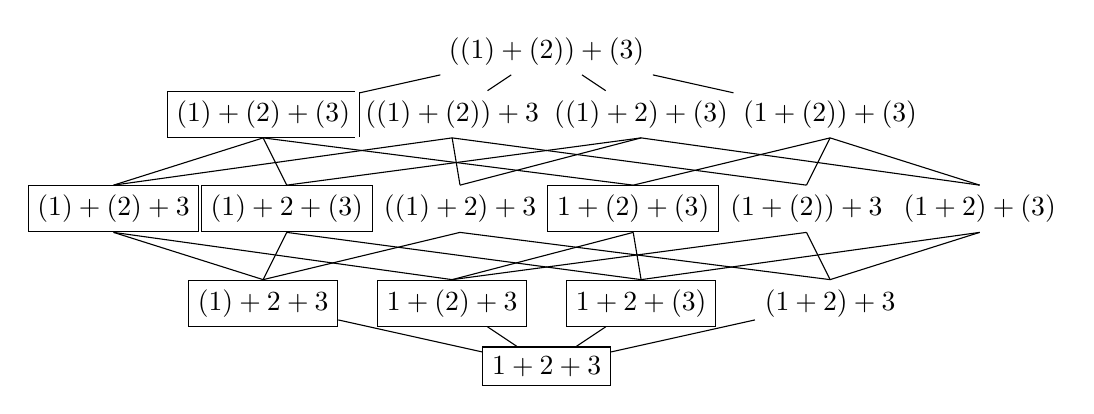
\begin{tikzpicture}[every node/.style={rectangle,draw}]
    \node (a) [draw=white] at (0,5) {$((1) + (2)) + (3)$};

    \node (b1) at (-3.6,4.2) {$(1) + (2) + (3)$};
    \node (b2) [draw=white] at (-1.2,4.2) {$((1) + (2)) + 3$};
    \node (b3) [draw=white] at ( 1.2,4.2) {$((1) + 2) + (3)$};
    \node (b4) [draw=white] at ( 3.6,4.2) {$(1 + (2)) + (3)$};

    \node (c1) at (-5.5,3) {$(1) + (2) + 3$};
    \node (c2) at (-3.3,3) {$(1) + 2 + (3)$};
    \node (c3) [draw=white] at (-1.1,3) {$((1) + 2) + 3$};
    \node (c4) at (1.1,3) {$1 + (2) + (3)$};
    \node (c5) [draw=white] at (3.3,3) {$(1 + (2)) + 3$};
    \node (c6) [draw=white] at (5.5,3) {$(1 + 2) + (3)$};

    \node (d1) at (-3.6,1.8) {$(1) + 2 + 3$};
    \node (d2) at (-1.2,1.8) {$1 + (2) + 3$};
    \node (d3) at ( 1.2,1.8) {$1 + 2 + (3)$};
    \node (d4) [draw=white] at ( 3.6,1.8) {$(1 + 2) + 3$};

    \node (e) at (0, 1) {$1 + 2 + 3$};

  \draw (e) -- (d1);
  \draw (e) -- (d2);
  \draw (e) -- (d3);
  \draw (e) -- (d4);

  \draw (d1.90) -- (c1.270);
  \draw (d1.90) -- (c2.270);
  \draw (d1.90) -- (c3.270);
  \draw (d2.90) -- (c1.270);
  \draw (d2.90) -- (c4.270);
  \draw (d2.90) -- (c5.270);
  \draw (d3.90) -- (c2.270);
  \draw (d3.90) -- (c4.270);
  \draw (d3.90) -- (c6.270);
  \draw (d4.90) -- (c3.270);
  \draw (d4.90) -- (c5.270);
  \draw (d4.90) -- (c6.270);

  \draw (c1.90) -- (b1.270);
  \draw (c1.90) -- (b2.270);
  \draw (c2.90) -- (b1.270);
  \draw (c2.90) -- (b3.270);
  \draw (c3.90) -- (b2.270);
  \draw (c3.90) -- (b3.270);
  \draw (c4.90) -- (b1.270);
  \draw (c4.90) -- (b4.270);
  \draw (c5.90) -- (b2.270);
  \draw (c5.90) -- (b4.270);
  \draw (c6.90) -- (b3.270);
  \draw (c6.90) -- (b4.270);

  \draw (b1) -- (a);
  \draw (b2) -- (a);
  \draw (b3) -- (a);
  \draw (b4) -- (a);
    %%   \draw[preaction={draw=white, -,line width=6pt}] (a) -- (e) -- (c);
  \end{tikzpicture}
  \caption{The lattice of words for the tree $a(a(n(1)+n(2))+n(3))$. The boxed words are shared with the lattice in Fig.~\ref{fig:lattice2}.}
  \label{fig:lattice1}
\end{figure}

Lemma~\ref{lemma:rangeset-equality} suggests a partition of the words in $\words(t)$ for any given $t \in L(T_D)$; group words $w'$ by their \emph{rangeset}, where $\rangeset(w') = \support(\rangebag(w'))$. These partitions can be partially ordered by subset on the rangeset, resulting in a lattice of word partitions per tree. This lattice is bounded, with top and bottom elements given by lemmas~\ref{lemma:possible-parentheses} and \ref{lemma:required-parentheses} respectively. Lemma~\ref{lemma:same-basic} further states that all words in $\words(t)$ share the same basic word. For example, Fig.~\ref{fig:lattice1} contains the lattice for the tree $a(a(n(1)+n(2))+n(3))$ (from our running example, defined in Fig.~\ref{fig:running-example-definition} on page~\pageref{fig:running-example-definition}). Each partition is represented by the word whose rangebag is a set. To reduce clutter, we do not draw the partitions that have grouping parentheses around the entire word. This outermost possible pair is uninteresting since it is always allowed, and would double the size of the figure if it was included.

\begin{figure}[t]

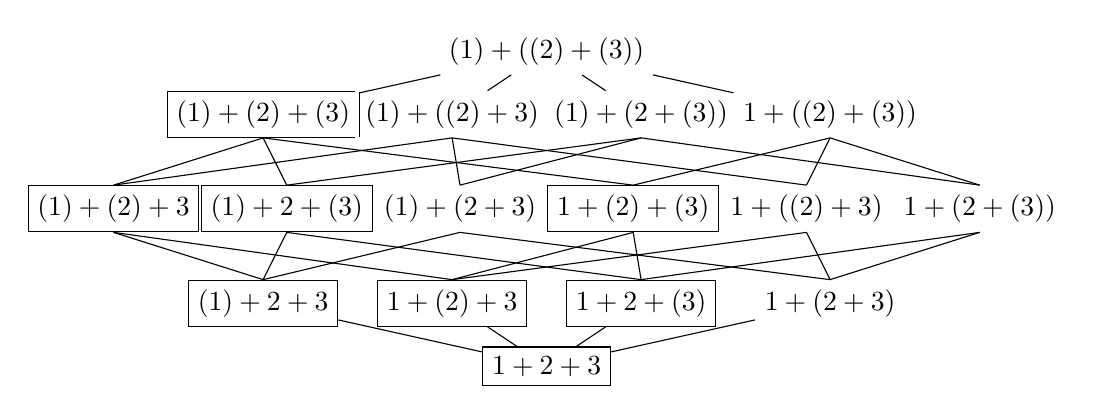
\begin{tikzpicture}[every node/.style={rectangle,draw}]
  \node (a) [draw=white] at (0,5) {$(1) + ((2) + (3))$};

  \node (b1) at (-3.6,4.2) {$(1) + (2) + (3)$};
  \node (b2) [draw=white] at (-1.2,4.2) {$(1) + ((2) + 3)$};
  \node (b3) [draw=white] at ( 1.2,4.2) {$(1) + (2 + (3))$};
  \node (b4) [draw=white] at ( 3.6,4.2) {$1 + ((2) + (3))$};

  \node (c1) at (-5.5,3) {$(1) + (2) + 3$};
  \node (c2) at (-3.3,3) {$(1) + 2 + (3)$};
  \node (c3) [draw=white] at (-1.1,3) {$(1) + (2 + 3)$};
  \node (c4) at (1.1,3) {$1 + (2) + (3)$};
  \node (c5) [draw=white] at (3.3,3) {$1 + ((2) + 3)$};
  \node (c6) [draw=white] at (5.5,3) {$1 + (2 + (3))$};

  \node (d1) at (-3.6,1.8) {$(1) + 2 + 3$};
  \node (d2) at (-1.2,1.8) {$1 + (2) + 3$};
  \node (d3) at ( 1.2,1.8) {$1 + 2 + (3)$};
  \node (d4) [draw=white] at ( 3.6,1.8) {$1 + (2 + 3)$};

  \node (e) at (0, 1) {$1 + 2 + 3$};

  \draw (e) -- (d1);
  \draw (e) -- (d2);
  \draw (e) -- (d3);
  \draw (e) -- (d4);

  \draw (d1.90) -- (c1.270);
  \draw (d1.90) -- (c2.270);
  \draw (d1.90) -- (c3.270);
  \draw (d2.90) -- (c1.270);
  \draw (d2.90) -- (c4.270);
  \draw (d2.90) -- (c5.270);
  \draw (d3.90) -- (c2.270);
  \draw (d3.90) -- (c4.270);
  \draw (d3.90) -- (c6.270);
  \draw (d4.90) -- (c3.270);
  \draw (d4.90) -- (c5.270);
  \draw (d4.90) -- (c6.270);

  \draw (c1.90) -- (b1.270);
  \draw (c1.90) -- (b2.270);
  \draw (c2.90) -- (b1.270);
  \draw (c2.90) -- (b3.270);
  \draw (c3.90) -- (b2.270);
  \draw (c3.90) -- (b3.270);
  \draw (c4.90) -- (b1.270);
  \draw (c4.90) -- (b4.270);
  \draw (c5.90) -- (b2.270);
  \draw (c5.90) -- (b4.270);
  \draw (c6.90) -- (b3.270);
  \draw (c6.90) -- (b4.270);

  \draw (b1) -- (a);
  \draw (b2) -- (a);
  \draw (b3) -- (a);
  \draw (b4) -- (a);
%%   \draw[preaction={draw=white, -,line width=6pt}] (a) -- (e) -- (c);
\end{tikzpicture}
\caption{The lattice of words for the tree $a(n(1)+a(n(2)+n(3)))$. The boxed words are shared with the lattice in Fig.~\ref{fig:lattice1}.}
\label{fig:lattice2}
\end{figure}

To show the connection between resolvable ambiguity and these lattices, consider the word ``\verb|1 + 2 + 3|''. It has two interpretations in our running example, $a(a(n(1)+n(2))+n(3))$, which we would normally write as \verb|(1 + 2) + 3|, and $a(n(1)+a(n(2)+n(3)))$, which we would normally write \verb|1 + (2 + 3)|. The lattices for these two trees are given in Figures~\ref{fig:lattice1} and \ref{fig:lattice2} respectively. The partitions that appear in both lattices are represented as boxed words, the others are unboxed. These shared partitions represent words that are ambiguous between these particular trees. Finding an unambiguous word is thus the same as finding a partition that is not shared with any other tree. In this particular case, there is no ambiguity with any other tree at all, and so the unboxed words are all valid resolutions of the ambiguity.

At this point it is clear that a given tree has an unambiguous word iff its lattice has at least one partition that is not shared with any other tree.

Next, we note that each lattice is uniquely determined by its top and bottom elements; it contains all elements between them:

\begin{lemma}
  Given $t \in L(T_D)$, $w'_\top, w'_\bot \in \words(t)$ such that $\forall w'.\ w' \in \words(t) => \rangebag(w'_\bot) \subseteq \rangeset(w') \subseteq \rangebag(w'_\top)$ the following holds:\\
  $\forall w'.\ \rangebag(w'_\bot) \subseteq \rangeset(w') \subseteq \rangebag(w'_\top) => w' \in \words(t)$. \label{lemma:top-bottom-determine}
\end{lemma}

\noindent Lemmas~\ref{lemma:possible-parentheses} and \ref{lemma:required-parentheses} guarantee the existence of two such words $w'_\top$ and $w'_\bot$.

Finally, we show the difference between versions~1 and 2 in the lattice setting: in version~1, the rangeset of the bottom word is the empty set:

\begin{lemma}
  In version~1, $rangeset(w'_\bot) = \emptyset$ for all trees, where $w'_\bot$ is given by Lemma~\ref{lemma:required-parentheses}. \label{lemma:version1-bot}
\end{lemma}

\noindent Since version~1 has no markings there are no required parentheses, thus the bottom word has no parentheses.

Our approach centers around finding a pair of lattices, such that one is entirely contained in the other. Since the former shares \emph{all} partitions with the latter, it has only ambiguous words, thus any of those words will be unresolvably ambiguous.

\begin{theorem}
  In versions~1 and 2, given a $t \in L(T_D)$ with a lattice determined by $w_\bot$ and $w_\top$, $\exists t' \in L(T_D).\ \basic(w_\bot) = \basic(w'_\bot) \land \rangeset(w_\bot) \subseteq \rangeset(w'_\bot) \land \rangeset(w'_\top) \subseteq \rangeset(w_\top) => \neg \exists w.\ \parse(w) = \{t\}$. \label{lemma:lattice-containment-implies-unresolvable}
\end{theorem}


\noindent For version~1, \emph{every} unresolvable ambiguity has this form:

\begin{theorem}
  In version 1, given a $t \in L(T_D)$ with a lattice determined by $w_\bot$ and $w_\top$, $\exists t' \in L(T_D).\ \basic(w_\bot) = \basic(w'_\bot) \land \rangeset(w'_\bot) \subseteq \rangeset(w_\bot) \land \rangeset(w_\top) \subseteq \rangeset(w'_\top) <=> \neg \exists w.\ \parse(w) = \{t\}$.
\end{theorem}

\begin{proof}
  The left-to-right implication is already given in Theorem~\ref{lemma:lattice-containment-implies-unresolvable}, and Lemma~\ref{lemma:version1-bot} together with $\basic(w_\bot) = \basic(w'_\bot)$ implies that $w_\bot = w'_\bot$. We thus need to show that $\neg \exists w.\ \parse(w) = \{t\} => \exists t' \in L(T_D).\ \basic(w_\bot) = \basic(w'_\bot) \land \rangeset(w'_\top) \subseteq \rangeset(w_\top)$.

  If all words in $\words(t)$ are ambiguous, then $\exists t' \in L(T_D).\ t' \neq t \land t' \in \parse(w_\top)$. Lemma~\ref{lemma:same-basic} gives $\basic(w_\bot) = \basic(w'_\bot)$. The definition of $w'_\top$ (Lemma~\ref{lemma:possible-parentheses}) gives $\rangeset(w_\top) \subseteq \rangebag(w'_\top)$, but since the rangebag of $w'_\top$ is a set, this also implies that $\rangeset(w_\top) \subseteq \rangeset(w'_\top)$.
\end{proof}

\subsection{A Lattice as a Word, and an Algorithm} \label{sec:lattice-vpl}

This section introduces a linear encoding of the lattices of the previous chapter as words. Lemmas~\ref{lemma:same-basic} and \ref{lemma:top-bottom-determine} imply that a lattice encoding requires three things: a basic word, a set of \emph{required} parentheses, and a set of \emph{possible} parentheses. We encode required parentheses with ``$\reqp{}$'' and possible parentheses with ``$\posp{}$''. For example, the lattice in Fig.~\ref{fig:lattice2} is represented by ``$\posp{\posp{1} + \posp{\posp{2} + \posp{3}}}$'', while the tree for ``$(1 + 2) * 3$'' has a lattice represented by ``$\posp{\reqp{\posp{1} + \posp{2}} * \posp{3}}$''. With this encoding we can apply the formidable body of knowledge available for word languages, albeit with some extra care; the linear encoding of a lattice is not unique.

For example, ``$\posp{\posp{1}}$'' and ``$\posp{1}$'' represent the same lattice, as do ``$\reqp{\posp{2}}$'' and ``$\reqp{2}$''. To gain uniqueness we forbid duplicated parentheses and prioritize required parentheses over possible parentheses, e.g., ``$\posp{\posp{1}}$'' is uniquely represented as ``$\posp{1}$'' while ``$\reqp{\posp{2}}$'' is uniquely represented as ``$\reqp{2}$''.

Lattice equality is now equvialent with equality of the linear encoding. To determine if a lattice is entirely contained in another, we make the following observation: we can move the top of the lattice ``up'' (new top rangeset is a strict superset) by adding a pair of possible parentheses, and move the bottom ``down'' (new bottom rangeset is a strict subset) by replacing a required pair with a possible pair. For example, ``$\reqp{1}2$'' is entirely contained in ``$\reqp{1}\posp{2}$'', which is entirely contained in ``$\posp{1}\posp{2}$''.

The centerpiece of our algorithm is a visibly pushdown automaton constructed in such a way that:

\begin{itemize}
\item There is a bijection between trees in $L(T_D)$ and successful runs.
\item The word recognized by a successful run is the linear encoding of the corresponding tree's lattice.
\end{itemize}

\noindent Two distinct successful runs through this automaton that recognize the same word thus imply two distinct trees that have exactly the same lattice. To detect lattices contained in each other, we create a modified copy, where the copy may add arbitrary (balanced, well-nested) possible parentheses, and replace any required pair of parentheses with a possible pair. The copy maintains much of the structure of the original, and in particular, keeps the connection to trees in $L(T_D)$ (though it is no longer a bijection: there are multiple successful runs per tree since there are multiple larger lattices). Two distinct successful runs, one in each automaton, that recognize the same word then imply two distinct trees where the lattice of one is entirely contained in the other.

We will now walk through the construction of this automaton, using the following language definition:

\begin{center}
\begin{tabular}{@{}l@{\quad$->$\quad}l@{ $:$\quad}l@{}}
  \toprule
  $E$ & $s$ & $E_{\{s\}}$ \verb|';'| $E$ \\
  $E$ & $v$ & \verb|'e'| \\
  \bottomrule
\end{tabular}
\end{center}

\noindent We first present a simplified construction that assumes no production can match a single non-terminal, i.e., for all right-hand side regular expressions $r$, $\neg \exists N_m.\ N_m \in L(r)$, to make the base idea easier to follow. Such cases introduce duplicated parentheses if handled in a naive way, and the extra book-keeping required to correctly handle them complicate this presentation, and will so be introduced after the more naive method.

Conceptually, each non-terminal represents a choice of which child production should replace it, and whether that production requires parentheses around it. We now make this explicit, to ensure that standard operations on finite automata produce the correct result. We replace each $N_m$ with a sum of the labels of productions in $N$, where each label has a subscript $\top$ or $\bot$ if parentheses are required or possible, respectively. For example, $E_{\{s\}}$ is replaced with $s_\top + v_\bot$.

\begin{center}
\begin{tabular}{@{}l@{\quad$->$\quad}l@{ $:$\quad}l@{}}
  \toprule
  $E$ & $s$ & $(s_\top + v_\bot)$ \verb|';'| $(s_\bot + v_\bot)$ \\
  $E$ & $v$ & \verb|'e'| \\
  \bottomrule
\end{tabular}
\end{center}

\noindent Next we construct a DFA per production. This can be done in the standard way by constructing an NFA, then determinizing it, and optionally minimizing it.

\begin{center}
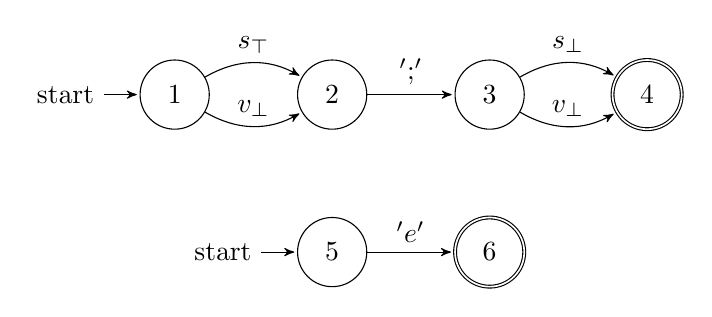
\begin{tikzpicture}[->,>=stealth',shorten >=1pt,auto,node distance=2cm,
    scale = 1,transform shape]

  \node[state,initial] (1) {$1$};
  \node[state] (2) [right of=1] {$2$};
  \node[state] (3) [right of=2] {$3$};
  \node[state,accepting] (4) [right of=3] {$4$};

  \node[state,initial] (5) [below of=2] {$5$};
  \node[state,accepting] (6) [right of=5] {$6$};

  \path (1) edge[bend left] node {$s_\top$} (2)
  (1) edge[bend right] node {$v_\bot$} (2)
  (2) edge node {$';'$} (3)
  (3) edge[bend left] node {$s_\bot$} (4)
  (3) edge[bend right] node {$v_\bot$} (4);
  \path (5) edge node {$'e'$} (6);

\end{tikzpicture}
\end{center}

\noindent We then combine them into a single visibly pushdown automaton. Every time we transition from a production to a child we push a symbol to the stack, which we then pop when we go back. We use $Q \times Q$ as our stack alphabet, to record the transition we are replacing in the parent. We thus replace every edge $p \xrightarrow{l_\top} q$, where $l \in \Labels$, with:

\begin{itemize}
  \item an edge $p \xrightarrow{'\reqpl', +(p, q)} p'$, where $p'$ is the initial state in the DFA corresponding to the production with label $l$, and
  \item an edge $q' \xrightarrow{'\reqpr', -(p, q)} q$ for every final state $q'$ in the DFA corresponding to the production with label $l$.
\end{itemize}

\noindent Similarly, for every edge $p \xrightarrow{l_\bot} q$, where $l \in \Labels$, we add edges $p \xrightarrow{'\pospl', +(p, q)} p'$ and $q' \xrightarrow{'\pospr', -(p, q)} q$.

Intuitively, we parse a child node with parentheses around it, then return. This is where our simplification is used, without it we might introduce double parentheses here.

\begin{center}
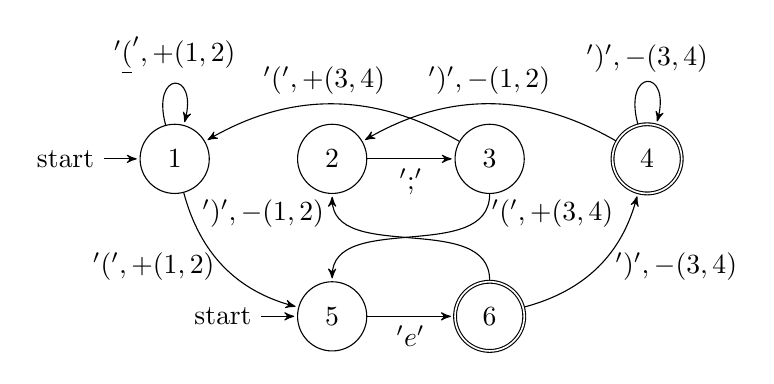
\begin{tikzpicture}[->,>=stealth',shorten >=1pt,auto,node distance=2cm,
    scale = 1,transform shape]

  \node[state,initial] (1) {$1$};
  \node[state] (2) [right of=1] {$2$};
  \node[state] (3) [right of=2] {$3$};
  \node[state,accepting] (4) [right of=3] {$4$};

  \node[state,initial] (5) [below of=2] {$5$};
  \node[state,accepting] (6) [right of=5] {$6$};

  \path (2) edge[below] node {$';'$} (3);
  \path (5) edge[below] node {$'e'$} (6);

  \path (1) edge[loop above] node{$'\reqpl', +(1, 2)$} (1)
  (4) edge[bend right, above] node{$'\reqpr', -(1, 2)$} (2);
  \path (1) edge[bend right, left] node{$'\pospl', +(1, 2)$} (5)
  (6) edge[left, in=270, out=90] node[xshift=-9.8mm,yshift=3mm]{$'\pospr', -(1, 2)$} (2);
  \path (3) edge[bend right, above] node[xshift=-1mm]{$'\pospl', +(3, 4)$} (1)
  (4) edge[loop above] node{$'\pospr', -(3, 4)$} (4);
  \path (3) edge[in=90, out=270, right] node[xshift=9mm,yshift=3mm]{$'\pospl', +(3, 4)$} (5)
  (6) edge[bend right, right] node[xshift=1mm]{$'\pospr', -(3, 4)$} (4);

\end{tikzpicture}
\end{center}

\noindent Finally, we add a new initial state and a new final state, and connect them with the initial and final states belonging to the starting non-terminal:

\begin{center}
\begin{tikzpicture}[->,>=stealth',shorten >=1pt,auto,node distance=2cm,
    scale = 1,transform shape]

  \node[state,initial] (7) [left of=5, xshift=-1.5cm] {$7$};
  \node[state,accepting] (8) [right of=6, xshift=1.5cm] {$8$};

  \node[state] (1) {$1$};
  \node[state] (2) [right of=1] {$2$};
  \node[state] (3) [right of=2] {$3$};
  \node[state] (4) [right of=3] {$4$};

  \node[state] (5) [below of=2] {$5$};
  \node[state] (6) [right of=5] {$6$};

  \path (2) edge[below] node {$';'$} (3);
  \path (5) edge[below] node {$'e'$} (6);

  \path (1) edge[loop above] node{$'\reqpl', +(1, 2)$} (1)
  (4) edge[bend right, above] node{$'\reqpr', -(1, 2)$} (2);
  \path (1) edge[bend right, left] node{$'\pospl', +(1, 2)$} (5)
  (6) edge[left, in=270, out=90] node[xshift=-9.8mm,yshift=3mm]{$'\pospr', -(1, 2)$} (2);
  \path (3) edge[bend right, above] node[xshift=-1mm]{$'\pospl', +(3, 4)$} (1)
  (4) edge[loop above] node{$'\pospr', -(3, 4)$} (4);
  \path (3) edge[in=90, out=270, right] node[xshift=9mm,yshift=3mm]{$'\pospl', +(3, 4)$} (5)
  (6) edge[bend right, right] node[xshift=1mm]{$'\pospr', -(3, 4)$} (4);

  \path (7) edge[bend left, left] node{$'\pospl', +(7, 8)$} (1)
  (7) edge[below] node{$'\pospl', +(7, 8)$} (5);
  \path (4) edge[bend left, right] node{$'\pospr', -(7, 8)$} (8)
  (6) edge[below] node{$'\pospr', -(7, 8)$} (8);

\end{tikzpicture}
\end{center}

\noindent The resulting pushdown automaton has only two sources of non-determinism: the edges labelled $'\pospl'$ and $'\reqpl'$. Each one corresponds to one of the allowable child productions at that point in the tree, thus there is one run per tree.

UNFINISHED

%% TODO: Continue here. Also figure out how to handle (E + E_m).

%% We now have a pushdown automaton (call it $A_{()}$) that recognizes the top word for each tree in $L(G_t)$. Next we need to be able to add arbitrary parentheses, to produce a word with a rangeset superset. To do this we create a copy of $A_{()}$ with one modification: for every state $s$ in $A_{()}$ (except the initial and final states), add two transitions $s \xrightarrow{'(', +p} s$ and $s \xrightarrow{')', -p} s$. To avoid cluttering the graph too much, these transitions are shown unlabeled below:

%% \begin{center}
%% \begin{tikzpicture}[->,>=stealth',shorten >=1pt,auto,node distance=2cm,
%%     scale = 1,transform shape]

%%   \node[state] (1) {$1$};
%%   \node[state] (2) [right of=1] {$2$};
%%   \node[state] (3) [right of=2] {$3$};
%%   \node[state] (4) [below of=1, xshift=1cm] {$4$};
%%   \node[state] (5) [right of=4] {$5$};
%%   \node[state,initial] (s) [left of=4] {};
%%   \node[state,accepting] (e) [right of=5] {};

%%   \draw
%%   (1) edge[loop, in=80, out=100, looseness=7] node{} (1)
%%   (1) edge[loop, in=70, out=110, looseness=6] node{} (1)
%%   (2) edge[loop, in=80, out=100, looseness=7] node{} (2)
%%   (2) edge[loop, in=70, out=110, looseness=6] node{} (2)
%%   (3) edge[loop, in=-10, out=10, looseness=7] node{} (3)
%%   (3) edge[loop, in=-20, out=20, looseness=6] node{} (3)
%%   (4) edge[loop, in=-80, out=-100, looseness=7] node{} (4)
%%   (4) edge[loop, in=-70, out=-110, looseness=6] node{} (4)
%%   (5) edge[loop, in=-80, out=-100, looseness=7] node{} (5)
%%   (5) edge[loop, in=-70, out=-110, looseness=6] node{} (5)
%%   (s) edge[left] node{$'(', +s$} (1)
%%   (s) edge[above] node{$'(', +s$} (4)
%%   (3) edge[right] node{$')', -s$} (e)
%%   (5) edge[above] node{$')', -s$} (e)
%%   (1) edge[above] node{$s$} (2)
%%   (4) edge[above] node{$z$} (5)
%%   (2) edge[bend left, below] node{$'(', +(2, 3)$} (1)
%%   (2) edge[bend left, left] node{$'(', +(2, 3)$} (4)
%%   (3) edge[loop above] node{$')', -(2, 3)$} (3)
%%   (5) edge[left, bend right] node{$')', -(2, 3)$} (3);

%% \end{tikzpicture}
%% \end{center}

%% \noindent We will call this automaton $A'_{()}$. Successful runs in this automaton have a surjection to runs in $A_($ (ignore transitions along the newly added edges), and thus also have a surjection to parse trees in $L(G_t)$. We can also note that every sucessful run in $A_{()}$ is also a successful run in $A'_{()}$, since the latter has all states and transitions of the former. Furthermore, two distinct runs, one in $A_{()}$ (call it $p$) and one in $A'_{()}$ (call it $p'$), that both recognize the same word must represent different parse trees in $L(G_t)$. To see why, we consider two cases:

%% \begin{enumerate}
%%   \item $p'$ only uses transitions present in $A_{()}$. This is a successful run in $A_{()}$, and distinct from $p$. But there is a bijection between runs in $A_{()}$ and parse trees in $L(T)$, thus $p'$ represents a different parse tree.
%%   \item $p'$ uses at least one transition added in $A'_{()}$. Using the surjection between runs in $A'_{()}$ and $A_{()}$ we find a new successful run that produces a different word (at least one fewer pair of parentheses). Since this run produces a different word, it must be distinct from $p$, and thus represent a different parse tree.
%% \end{enumerate}

%% \noindent Two distinct successful runs that accept the same word thus represent two trees where one permits a superset rangeset of the other. To find such runs we construct a product automaton and trim it. We can construct a product automaton since both $A_{()}$ and $A'_{()}$ are visibly pushdown, with the same partition of the input alphabet (push on open parenthesis, pop on close parenthesis, do nothing otherwise). We can trim the product since it retains the same partitioning and thus is also visibly pushdown.

%% In this product automaton, if any transition pushes a stack symbol $(a, b)$ where $a \neq b$, or transitions to a state $(p, q)$ where $p \neq q$, then there is a successful run that corresponds to two distinct runs through $A_{()}$ and $A'_{()}$ (since the automaton is trim).

\begin{theorem}
  There is a bijection between successful runs in $A_{\posp{}}$ and trees $t \in L(T_D)$.
\end{theorem}

\begin{proof}
  (These are two attempts at showing the same thing, next attempt starts at ``Proof sketch''. I would strongly suggest reading ``Formal stuff'' first.)
  $A_{\posp{}}$ has a single initial state, and a single final state, call them $s$ and $f$ respectively. The two are distinct, and $f$ is reachable only through transitions that pop a stack symbol with $s$ and $f$ as the two first components. Transitions that push such symbols originate in $s$, and no other transitions originate in $s$. Thus all successful runs start in configuration $(s, \epsilon)$ and end in $(f, \epsilon)$, whereby every pushing transition in the run can be paired with a corresponding popping transition. We will now construct a tree $t \in L(T_D)$ in a bottom-up fashion.

  Select a subsequence of the run $R = (s, \epsilon) \; R_1 \; (p, s) \xrightarrow{a, +(p, q, w)} (p', (p, q, w) \cdot s) \; R_2 \; (q', (p, q, w) \cdot s \xrightarrow{b, -(p, q, w)} (q, s) \; R_2 \; (f, \epsilon)$ such that $R_2$ contains no pushing or popping operations. The only transitions that leave the stack unchanged in $A_{\posp{}}$ come from DFAs generated from productions in $D$. There is no way to transition between two such DFAs without using a pushing or popping transition, thus $R_2$ must be a successful run in the DFA for some labelled production $N -> l : r$ in $D$. $T_D$ must contain a corresponding production $N -> l(r)$. Now consider the sequence of input symbols $w'$ along the transitions in $R_2$. We have $w' \in L(r)$, since $R_2$ is a successful run in a DFA constructed from $r$. Thus $l(w') \in L_N(T_D)$. Now add parent nodes to this subtree for every label in $w$, e.g., if $w = l_1 \cdot l_2 \cdot l_3$ construct $l_1(l_2(l_3(l(w'))))$. We can then replace the subsequence of $R$ with this subtree, and then repeat the process until we have a tree with root $l'$, where $D$ has a labelled production $S -> l': r'$ for some $r'$ and the starting symbol $S$.

  To construct a successful run from a tree $t \in L(T_D)$ we can traverse the tree in a preorder, while at the same time constructing a run in $A_{\posp{}}$ starting from $(s, \epsilon)$. If the next terminal is in $\T$, i.e., a strictly zero-arity terminal, we take a transition originating in a DFA, which must be unique. If the next terminal is in $\Labels$, i.e., an unranked terminal, we take one of the added edges. However, this choice of edge might not be unique: there may be multiple edges from the current state to an appropriate DFA initial state. These stem from the original DFA having two transitions from the same state with the same label but different subscripts, e.g., $p \xrightarrow{l_\bot} q$ and $p \xrightarrow{l_\top} q'$. However, if both of these transitions were valid choices for the current tree that would imply that the DFA for that level can recognize two distinct words that differ only in subscripts. But distinctly subscripted terminals must originate from distinct occurances of marked non-terminals (since a $\top$ subscript corresponds to a mark, and a $\bot$ subscript corresponds to the absence of a mark), which would imply that the original regular expression is ambiguous if the marks are removed, which we explicitly ruled out in Section~\ref{sec:parse-time-disambiguation}.

  Proof sketch: to go from a successful run to a tree $t \in L(T_D)$: by construction, all successful runs must begin and end with an empty stack. Every pushing transition can thus be paired with a popping transition in the run. We can construct a tree in a bottom-up fashion by replacing every such pair with a tree $l_1(l_2(\ldots l_n(x)\ldots))$, where $x$ is the sequence of terminals and/or trees between the pair, the terminals $l_1, l_2, \ldots, l_{n-1}$ stem from the third component of the pushed stack symbol ($l_1 \cdots l_{n-1}$), and $l_n$ is the label of the production whose DFA the pushing transition ends in.

  For the inverse direction we construct a run by traversing the tree in a preorder\footnote{Where we also keep track of when we ``go back up'' the tree.}. Terminals in $\T$ cause transitions internally in a DFA, while terminals in $\Labels$ cause a pushing transition (and later a corresponding, unique popping transition) to the initial state of the DFA corresponding to the production with that label. Note that a sequence of terminals in $\Labels$ that have only a single child (which is also in $\Labels$) cause only one transition, all terminals but the last end up in the third component of the pushed stack symbol. The choice of pushing transition is \emph{not} unique however; there may be multiple available transitions that differ in the recognized input symbol and the second component of the pushed stack symbol, neither of which are necessarily determined by the shape of the tree. This non-determinism does not introduce multiple successful runs however, since two such runs would imply the existence of two distinct runs through the DFA corresponding to some labelled production that recognize the same word, except with different subscripts. But two otherwise equal terminals with different subscripts must originate from different occurrences of marked non-terminals in the original regular expression (since a $\top$ subscript represents a mark, and a $\bot$ subscript represents the absence of a mark), thus that regular expression must be ambiguous after all marks are removed. But Section~\ref{sec:parse-time-disambiguation} explicitly ruled this out, thus only one of the pushing transitions can be a valid choice.

% TODO: technically, we should perhaps mention that these two constructions are inverses of each other, but that's relatively easy to see once you understand them.
\end{proof}

\subsubsection{Formal Stuff}

Given a language definition $D$, with terminals $\T$, labels $\Labels$, and starting non-terminal $S$. Construct two functions $\dfa : \Labels -> \mathit{DFA}(\T \cup (\Labels \times \{\top, \bot\})$ and $\passthrough : \Labels -> 2^{\Labels \times \Labels \times \{\top, \bot\} \times \Labels^{*}}$:

\begin{description}
\item[$\dfa(l)$:] Given the production $N -> l : r$, compute the regular language $L' := L(r) \setminus \{N'_m \mid N' \in \NT, m \subseteq \Labels\}$. Then replace every marked non-terminal $N'_m$ with the regular expression $l_{1l_1 \in m} + l_{2l_2 \in m} + \ldots + l_{nl_n \in m}$, where $l_i$ are all the labels of productions $N' -> l_i : r_i$, e.g., $E_{\{a\}}$ in the running example would be replaced by $l_\bot + a_\top + m_\bot + n_\bot$. Then construct a DFA for this language.

\item[$\passthrough(l)$:] Given a production $N -> l : r$, this is the set $\{(l, l, \bot, \epsilon)\} \cup \{(l, l', l' \in m, l) \mid \nt(l') = N', N'_m \in L(r)\}$.
\end{description}

\noindent Compute the set $P$ as the closure of $\bigcup_l \passthrough(l)$ using the following operation:

$$ (l_1, l_2, r_1, w_1) \cdot (l_2, l_3, r_2, w_2) = (l_1, l_3, r_1 \lor r_2, w_1 \cdot w_2) $$

\noindent $P$ is finite if $D$ has no cycles $N =>^{+} N$\footnote{This is notation from CFGs, which is semi-obvious what it means, but technically not defined here.}. Such a cycle is easy to detect (depth-first search), and means that any tree that contains a production from the non-terminal $N$ only ever produces infinitely ambiguous words, i.e., all words for such a tree are unresolvably ambiguous.

Given $\dfa(l) = (Q_l, \T \cup (\Labels \times \{\top, \bot\}), \delta_l, s_l, F_l)$ for all $l \in Labels$, and $\nt(l) = N$ iff $(N -> l : r) \in D$, construct a VPDA $A_{\posp{}} = (Q, \T', \Gamma, \delta, s, \{f\})$ where:

\begin{itemize}
\item $s$ and $f$ are two new distinct states.
\item $Q = \{s, f\} \cup \bigsqcup_l Q_l$.
\item $\T' = \T \cup \{\reqpl, \pospl, \pospr\}$.
\item $\Gamma = Q \times Q \times \Labels^{*}$.
\item $\delta$ is defined by (in hindsight this should probably be written as constructing a set $\delta$, i.e., instead of a function $\delta: Q \times \T' \times (\Gamma \cup \{\lambda\}) -> 2^{Q \times (\Gamma \cup \{\lambda\})}$ we have a set $\delta \subseteq Q \times \T' \times (\Gamma \cup \{\lambda\}) \times Q \times (\Gamma \cup \{\lambda\})$, would probably be easier to read):
  $$
  \begin{array}{r@{\;=\;}l@{\;\mid\;}l}
    \delta(p, a, \lambda)
    & \multicolumn{2}{@{}l@{}}{\{(\delta_l(p, a), \lambda)\} \qquad \text{ where } p \in Q_l \text{ and } a \in \T} \\

    \delta(p, \text{``}\reqpl\text{''}, \lambda)
    & \{ (s_{l_3}, (p, q, w))
    & p \in Q_{l_1}, \delta_{l_1}(p, (l_2, r_1)) = q, (l_2, l_3, r_2, w) \in P, r_1 \lor r_2 \} \\

    \delta(p, \text{``}\pospl\text{''}, \lambda)
    & \{ (s_{l_3}, (p, q, w))
    & p \in Q_{l_1}, \delta_{l_1}(p, (l_2, r_1)) = q, (l_2, l_3, r_2, w) \in P, \neg (r_1 \lor r_2) \} \\

    \delta(f_{l_3}, \text{``}\reqpr\text{''}, (p, q, w))
    & \{ (q, \lambda)
    & p \in Q_{l_1}, \delta_{l_1}(p, (l_2, r_1)) = q, (l_2, l_3, r_2, w) \in P, f_{l_3} \in F_{l_3} \} \\

    \delta(s, \text{``}\reqpl\text{''}, \lambda)
    & \{ (s_{l_2}, (s, f, w))
    & \nt(l_1) = S, (l_1, l_2, \top, w) \in P \} \\

    \delta(s, \text{``}\pospl\text{''}, \lambda)
    & \{ (s_{l_2}, (s, f, w))
    & \nt(l_1) = S, (l_1, l_2, \bot, w) \in P \} \\

    \delta(f_{l_2}, \text{``}\reqpr\text{''}, (s, f, w))
    & \{ (f, \lambda)
    & nt(l_1) = S, (l_1, l_2, r, w) \in P, f_{l_2} \in F_{l_2}\} \\
  \end{array}
  $$
\end{itemize}

\noindent We also construct a modified VPDA $A'_{\posp{}} = (Q, \T', \Gamma \cup \{\gamma\}, \delta', s, \{f\})$ where:

\begin{itemize}
\item $\gamma$ is a new distinct stack symbol.
\item $\delta'(p, a, g) = \delta(p, a, g) \cup \delta''(p, a, g)$, where $\delta''$ is given by:
  $$
  \begin{array}{r@{\;=\;}l@{}}
    \delta''(p, \text{``}\pospl\text{''}, \lambda)
    & \{ (p, \gamma) \} \\

    \delta''(p, \text{``}\pospr\text{''}, \gamma)
    & \{ (p, \lambda) \} \\

    \delta''(p, \text{``}\pospl\text{''}, \lambda)
    & \delta(p, \text{``}\reqpl\text{''}, \lambda) \\
  \end{array}
  $$
\end{itemize}

\noindent To find two distinct successful runs, one in each automaton, that recognize the same word we construct the product automaton $A_{\posp{}} \times A'_{\posp{}} = (Q \times Q, \T', \Gamma \times (\Gamma \cup \{\gamma\}), \delta_{\times}, (s, s), \{(f, f)\})$, where $\delta_{\times}$ is given in Section~\ref{sec:preliminaries-vpls} (using the partitions $\T_c = \{ \reqpl, \pospl \}$, $\T_i = \T$, and $\T_r = \{\reqpr\}$). If the product automaton has a successful run that passes through at least one configuration $((p, p'), (g, g')\cdot w)$ such that $p \neq p' \lor g \neq g'$, then that run corresponds to two distinct runs in $A_{\posp{}}$ and $A'_{\posp{}}$. We check for the existence of such a run by trimming the product automaton and looking for a transition that pushes $(g, g')$ where $g \neq g'$, or transitions to $(q, q')$ where $q \neq q'$.

Performing this procedure directly on a language definition $D$ gives a sound decision procedure where the presence of two distinct runs implies unresolvably ambiguous. If we instead do it on a modified $D$ with no marks on the right hand side of any production (i.e., all non-terminals have the form $N_\emptyset$) we get a sound decision procedure where the absence of two distinct runs implies resolvably ambiguous.

There are thus cases where we can answer resolvably ambiguous or unresolvably ambiguous with certainty, and cases where we cannot answer either way with certainty.

\section{Dynamic Resolvability Analysis} \label{sec:dynamic}

The dynamic resolvability problem is as follows: for a given $w' \in L(G'_D)$ determine whether $\forall t \in \parse(w').\ \exists w'_2.\ \parse(w'_2) = \{t\}$. Furthermore, for practical reasons, if the word is resolvably ambiguous we wish to produce a (minimal) witness for each tree. Additionally, while Section~\ref{sec:static} requires a language definition $D$ to not contain parentheses, this section merely requires parentheses to be balanced.

Our approach centers around around $\words(t)$, which, being a set of words, can be considered a language in the classical sense. Each such language turns out to be a visibly pushdown language. Given a set of trees in $L(T_D)$ we can construct a corresponding set of non-overlapping visibly pushdown automata (i.e., each automaton only accepts words not accepted by any other automaton) since VPLs are closed under complement and intersection \cite{alurVisiblyPushdownLanguages2004}. These automata can then be examined to determine if they accept the empty language (which implies that the corresponding tree only has ambiguous words), or otherwise produce a witness, a word accepted only by that automaton.

For this section, we assume the presence of a single language definition $D$ with terminals in $\T$, labels in $\Labels$, and non-terminals in $\NT$.

\begin{theorem}
  Given a $t \in L(T_D)$, we can construct a visibly pushdown automaton that accepts exactly $\words(t)$.
\end{theorem}

\noindent We construct this automaton in a bottom-up fashion. A sequence of terminals in $\T$ is easily recognized by a sequence of transitions that do not interact with the stack. Each subtree allows surrounding grouping parentheses, which can be represented by transitions that push and pop stack symbols (one unique stack symbol per subtree), to ensure that they are balanced. With that, there are two remaining complications: a subtree $l(w)$ recognized from a marked non-terminal $N_m$ where $l \in m$ must have one or more surrounding parentheses instead of zero or more, and we must maintain the visibly pushdown property, i.e., all transitions labelled ``$($'' or ``$)$'' must push or pop stack symbols, respectively. The former can be solved by either tracking the subtree's origin when parsing, or reparsing with the right hand side regular expression, while the latter is solved by introducing a new stack symbol $\gamma$ that is pushed and popped by all non-grouping parenthesis terminals. Writing the transition function $\delta : Q \times \T \times (\Gamma \cup \{\lambda\}) -> 2^{Q \times (\Gamma \cup \{\lambda\})}$ as a subset of $Q \times \T \times (\Gamma \cup \{\lambda\}) \times Q \times (\Gamma \cup \{\lambda\})$, and using $\sqcup$ for disjoint union:

$$
\begin{array}{r@{\;}l}
  f(a)
  & = \begin{cases}
    (\{p, q\}, \T, \emptyset, \{(p, a, \lambda, q, \lambda)\}, p, \{q\})
    & \text{if } a \notin \{\text{``}(\text{''}, \text{``})\text{''}\} \\

    (\{p, q\}, \T, \{\gamma\}, \{(p, \text{``}(\text{''}, \lambda, q, \gamma)\}, p, \{q\})
    & \text{if } a = \text{``}(\text{''} \\

    (\{p, q\}, \T, \{\gamma\}, \{(p, \text{``})\text{''}, \lambda, q, \lambda))\}, p, \{q\})
    & \text{if } $a = \text{``})\text{''}$ \\
  \end{cases} \\

  f(w_1 \cdot w_2)
  & = (Q_1 \sqcup Q_2, \T, \Gamma', \delta_1 \cup \delta_2 \cup \{(f_1, \lambda, \lambda, s_2, \lambda)\}, s_1, \{f_2\}) \\
  & \text{ where } f(w_i) = (Q_i, \T, \Gamma_i, \delta_i, s_i, \{f_i\}) \\
  & \hphantom{\text{ where }} \Gamma' = (\Gamma_1 \setminus \{\gamma\}) \sqcup (\Gamma_2 \setminus \{\gamma\}) \cup \{\gamma\} \\

  f(l(w))
  & = \begin{cases}
    (Q \sqcup \{p, q\}, \T, \Gamma', \delta \cup \delta_1, p, \{q\}) & \text{if $l$ is marked in the introducing non-terminal.} \\
    (Q, \T, \Gamma', \delta \cup \delta_2, s, \{f\}) & \text{if $l$ is unmarked in the introducing non-terminal.} \\
  \end{cases} \\
  & \text{ where } f(w) = (Q, \T, \Gamma, \delta, s, \{f\}) \\
  & \hphantom{\text{ where }} \Gamma' = (\Gamma \setminus \{\gamma\}) \sqcup \{g, \gamma\} \\
  & \hphantom{\text{ where }} \delta_1 = \{(p, \text{``}(\text{''}, \lambda, p, g), (p, \text{``}(\text{''}, \lambda, s, g), (f, \text{``})\text{''}, g, q, \lambda), (q, \text{``})\text{''}, g, q, \lambda)\} \\
  & \hphantom{\text{ where }} \delta_2 = \{(s, \text{``}(\text{''}, \lambda, s, g), (f, \text{``})\text{''}, g, f, \lambda)\} \\
\end{array}
$$

UNFINISHED

\section{Case Studies} \label{sec:evaluation}

% TODO: Make sure that forbids are explained

We have implemented a tool and a small DSL for syntax definition
that generates a language definition in the style of
Section~\ref{sec:parse-time-disambiguation}, which the tool then
uses to construct a parser and do dynamic resolvability analysis.
The tool is implemented in Haskell and uses an off-the-shelf
implementation\footnote{\url{http://hackage.haskell.org/package/Earley}}
of the Earley parsing algorithm
\cite{earleyEfficientContextfreeParsing1970}. The purpose of these
case studies is to showcase possible use cases of resolvable
ambiguity in the context of composing separately defined DSLs (a
subset of Orc, Section~\ref{sec:evaluation-orc}), and of defining
a pre-existing general purpose programming language (OCaml,
Section~\ref{sec:evaluation-ocaml}.

The syntax definition DSL builds on the ``syncons'' introduced by
\citet{palmkvistCreatingDomainSpecificLanguages2019}, wherein each
production is defined separately from each other (one
\syncon{syncon} each).
%
The main difference between the DSL and the formalism in
Section~\ref{sec:parse-time-disambiguation} is that marks are
introduced as separate \syncon{forbid} declarations rather than
inline in productions. This allows supporting high-level
convenience constructs, e.g., specifying precedence between
previously defined operators instead of manually inserting marks,
but is also important for composability as ambiguities can be
statically resolved without changing the original definitions.
Other convenience constructs include defining prefix, infix and
postfix operators with a given associativity.

The running example used in
Section~\ref{sec:parse-time-disambiguation}
(Fig.~\ref{fig:running-example-definition} on
page~\pageref{fig:running-example-definition}) can be defined as
follows:

\begin{tabular}{ll}
\begin{lstlisting}[language=syncon,boxpos=t]
type Exp
grouping "(" Exp ")"
precedence {
  mul; // higher in precedence list
  add; // means higher precedence
}
\end{lstlisting}
&
\begin{lstlisting}[language=syncon,boxpos=t]
token Integer = "[0-9]+"
syncon literal: Exp = n:Integer
syncon list: Exp =
  "[" (head:Exp (";" tail:Exp)*)? "]"
infix add: Exp = "+"
infix mul: Exp = "*"
\end{lstlisting}
\end{tabular}\smallskip

\noindent Here, we define a syntax type \syncon{Exp} for
expressions, and declare that parentheses can be used to group
expressions. We define a lexical token for integers, and a
\syncon{syncon} for integer literals using this token. A list is
defined as a sequence of zero or more expressions separated by
semi-colons wrapped in square braces. Finally, addition and
multiplication is defined as infix syncons with the expected
precedence rules. Note that we could just as well have replaced
the precedence list with explicit \syncon{forbid} declarations,
``\syncon{forbid mul.left = add}'' and ``\syncon{forbid mul.right = add}''
(cf. the mark $\{a\}$ in the production of $m$ in
Fig.~\ref{fig:running-example-definition}).

% If marks are needed in non-precedence related
% situations, e.g., adding sequential composition to the running
% example, they can be introduced with ``forbids'':

% \begin{lstlisting}[language=syncon]
% infix seqComp: Exp = ";"
% forbid list.head = seqComp
% forbid list.tail = seqComp
% \end{lstlisting}

\subsection{Composing Language Definitions} \label{sec:evaluation-orc}

In this section, we consider the use case of defining a language
and composing it with another previously defined language, showing
how we can deal with the resulting ambiguities that arise from the
composition.
%
The language being defined is a subset of
Orc~\cite{kitchinOrc2009}, a functional programming language which
includes a number of special-purpose combinators for coordinating
concurrent workflows. On their own, these combinators act as a DSL
for concurrency.

In Orc, every expression can ``publish'' zero or more values. Orc
defines four combinators for orchestrating these published values:
the parallel (\ocaml{|}), sequential (\ocaml{>}$x$\ocaml{>}),
pruning (\ocaml{<}$x$\ocaml{<}), and ``otherwise'' (\ocaml{;})
combinators.
%
The expression $e_1$ \ocaml{|} $e_2$ runs $e_1$ and
$e_2$ in parallel, publishing any value published by either of
them.
%
The expression $e_1$ \ocaml{>}$x$\ocaml{>} $e_2$ executes
$[x\mapsto v]e_2$ for \emph{each} value $v$ published by $e_1$,
building a concurrent pipeline.
%
The expression $e_1$ \ocaml{<}$x$\ocaml{<} $e_2$ executes
$[x\mapsto v]e_1$ for \emph{first} value $v$ published by $e_2$
(discarding any remaining values published by $e_2$).
%
Finally, $e_1$\ocaml{;}$e_2$ runs $e_2$ only if running $e_1$ does
not publish any values.

The syncon definition of the Orc combinators is very simple (the
precedence rules follow the original
definition~\cite{kitchinOrc2009}):

\begin{tabular}{ll}
\begin{lstlisting}[language=syncon,boxpos=t]
type Exp
grouping "(" Exp ")"
precedence {
  seq; par; prune; otherwise;
}
\end{lstlisting}
&
\begin{lstlisting}[language=syncon,boxpos=t]
token Ident = "[[:lower:]][[:word:]]*"
infix par:Exp = "|"
infix seq:Exp = ">" x:Ident ">"
infix prune:Exp = "<" x:Ident "<"
infix otherwise:Exp = ";"
\end{lstlisting}
\end{tabular}\smallskip

\noindent
Na\"{i}vely composing this definition with another, separately
defined language is likely to introduce ambiguities. For example,
if that language also contains infix operators, the precedence
between these and the Orc combinators will be undefined. With
support for resolvable ambiguity however, we can allow this
ambiguity and let programmers disambiguate expressions using
parentheses. After composing the above definition with a simple
language supporting addition, variables, and function calls
(language definition omitted for brevity), parsing the expression
%
``\ocaml{1 + 2 >x> f(x)}''
%
results in the following error message from our tool:

\begin{lstlisting}[language={[objective]caml}]
Ambiguity error with 2 alternatives:
  ( 1 + 2 ) > x > f ( x )
  1 + ( 2 > x > f ( x ) )
\end{lstlisting}

\noindent
Because there is no precedence specified between \ocaml{+} and
\ocaml{>x>}, disambiguation is required to specify the order of
operations.
%
In this case, it is likely that the preferred semantics is to have
all operators in the base language bind tighter than the Orc
combinators, and these precedence rules can be added after the
composition without changing the original definitions. Importantly
though, we are not \emph{required} to resolve this ambiguity at
time of composition.

Because of how we defined the syntax of the combinators, and since
parsing with the tool is currently whitespace insensitive, the
multi-character combinators (sequencing and pruning) are parsed as
three separate lexical tokens (this is visible in how whitespace
is inserted in the error message above). This means we can also
run into \emph{unresolvable} ambiguities, for example if our base
language includes comparison of numbers with \ocaml{<} and
\ocaml{>}. With such a base language (assuming no associativity
for \ocaml{>}), parsing the expression
%
``\ocaml{42 >x> f(x)}''
%
will result in the following error message:

\begin{lstlisting}[language={[objective]caml}]
Unresolvable ambiguity error with 2 alternatives.
\end{lstlisting}

\begin{minipage}{.3\textwidth}
\begin{lstlisting}[language={[objective]caml}]
Resolvable alternatives:
  ( 42 > x ) > f ( x )
  42 > ( x > f ( x ) )
\end{lstlisting}
\end{minipage}
\hfill
\begin{minipage}{.5\textwidth}
\begin{lstlisting}[language={[objective]caml}]
Unresolvable alternatives:
  seq
   - int                  gt.orc:1:1-3
   - call                 gt.orc:1:8-12
\end{lstlisting}
\end{minipage}

\noindent
By adding parentheses, a programmer can disambiguate the
expression as two comparisons. However, there is no way for a
programmer to specify that what they want is a sequential
combinator with left and right children being an integer and a
function call respectively. In this case we have at least three
choices to make as language designers:

\begin{itemize}
\item We could decide to forbid the case where two comparisons are
  right next to each other, e.g., \syncon{forbid gt.left = gt} and
  \syncon{forbid gt.right = gt} (where \syncon{gt} is the syncon
  for the greater-than operator).
\item We could change the definition of the parallel combinators
  and define separate lexical tokens for the combinators, e.g.,
  \syncon{token Seq = ">[[:lower:]][[:word:]]*>"}. This would add
  just enough whitespace sensitivity to allow separating the
  different cases.
\item We could change the syntax of the combinators completely to
  avoid clashes with other operators.
\end{itemize}

\noindent
The change in the first alternative is somewhat ad-hoc, but can be done after composition
and would allow us to reuse both language definitions without
modifications. In the latter two alternatives, we lose reuse of
the definitions of Orc combinators, but place no additional
restrictions on the base language. The preferred resolution
strategy is likely to differ between different compositions and
different languages.
%
For example, another unresolvable ambiguity is going to show up if
the base language uses semi-colons, e.g. for sequencing
expressions (this would clash with the ``otherwise'' combinator).
In this case, there is no reasonable way to disambiguate
``\ocaml{e1; e2}'' without changing the syntax of one of the
operations.

The main takeaway from this case study is that resolvable
ambiguity makes composition of languages less restrictive than if
all ambiguity is completely banned. The approach is strictly more
general since dynamic resolvability analysis allows deferring
disambiguation to the programmer, while removing ambiguities from
the resulting grammar is also possible.


\subsection{Applying Resolvable Ambiguity to a Full Language} \label{sec:evaluation-ocaml}

The syncon definition of the OCaml language includes most syntax described in chapters 7 and 8 in the OCaml reference manual (the base language and extensions, respectively) and is sufficient to parse roughly 75\% (1012 out of 1334 files) of the \verb|.ml| files present in the OCaml compiler itself. The definition is just under 700 lines, excluding comments and empty lines (just over 1000 lines otherwise). It has been written to be as close to the grammar presented in the reference manual as possible, but with additions to conform to how the canonical compiler behaves on cases that are underspecified in the manual.

The failing cases stem from three different causes:

\begin{itemize}
\item As of yet unspecified syntax. Due to a lack of time there are still parts of the language that we have not yet implemented. These appear solvable, but we can of course not be sure until we do.
\item Our system does not support specifying ``longest match'' on a production, which is required to handle the pattern matching constructs correctly. We can handle some of these cases with marks, but not all.
\item Different definitions of precedence. Our translation from precedence to marks is shallow, it only considers direct children, but OCaml has deep precedence. For example, addition binds stronger than \ocaml{if} (which syntactically functions as a prefix operator in OCaml), thus
  \begin{lstlisting}[language={[objective]caml}]
  1 + let x = 1 in x + 2
  \end{lstlisting}
  should be parsed as
  \begin{lstlisting}[language={[objective]caml}]
  1 + (let x = 1 in (x + 2))
  \end{lstlisting}
  while our tool presents the following ambiguity error message:
  \begin{lstlisting}[language={[objective]caml}]
Ambiguity error with 2 alternatives:

  1 + ( let x = 1 in x ) + 2
  1 + let x = 1 in ( x + 2 )
  \end{lstlisting}
  The former alternative is perhaps more easily understood as
  \begin{lstlisting}[language={[objective]caml}]
  (1 + (let x = 1 in x)) + 2
  \end{lstlisting}
  Looking at this tree, two levels at a time, we see ``\ocaml{(_ + _) + 2}'', ``\ocaml{1 + let _ in _}'', and ``\ocaml{let x = 1 in x}'', all of which are individually precedence correct.
\end{itemize}

The various definitions in the syncon OCaml definition are organized by the chapter in the reference manual that introduces them, plus an appendix with additions and changes required to mimic the behavior of the canonical compiler. Many of these are strict additions, requiring no changes to previous syncons, but not all. For example, OCaml allows placing ``attributes'' on most syntactical constructs in the language, extra information visible to tools but otherwise without semantic meaning. These can be written with an ``infix'' notation right after the keyword that introduces the syntactical construct, e.g., \ocaml{let[@foo] x = 1 in x}. This syntax is not fully specified; the manual merely contains seven examples, while the testsuite uses this syntax in roughly 50 different constructs. All these cases require changes to the original syncon definitions, making them slightly more complicated than the manual suggests them to be upon their introduction.

% \subsection{Cyphym} \label{sec:evaluation-cyphym}

\section{Related Work}

\citet{afroozehSafeSpecificationOperator2013}'s operator ambiguity removal patterns bear a striking resemblance to the marks presented in this paper. However, in special-casing (what in this paper would be) marks on left and right-recursions in productions they correctly cover the edge case discussed in Section~\ref{sec:evaluation-ocaml}. This approach thus suggests an interesting direction for future work: to integrate it into a system designed around resolvable ambiguity, and extending the algorithms presented in this paper to cover it.

\citet{danielssonParsingMixfixOperators2011} give a method for specifying grammars for expressions containing mixfix operators. They allow non-transitive, non-total precedence, and ``feel that it is overly restrictive to require the grammar to be unambiguous.'' Similar to our approach, they do not reject ambiguous grammars, only ambiguous parses. They also introduce a concept of \emph{precedence correct} expressions; expressions where direct children must be related by precedence (children must have higher precedence than parents). This is more restrictive than our approach, e.g., in a language where \verb|'+'| and \verb|'-'| have no defined relative precedence they reject \verb|'1 + 2 * 3'| as syntactically invalid, while we parse it as an ambiguous expression.

Silver \cite{vanwykSilverExtensibleAttribute2010}, a system for defining extensible languages using attribute grammars, and its associated parser Copper \cite{} have a ``Modular Well-Definedness Analysis'' \cite{kaminskiModularWellDefinednessAnalysis2013}, with which extension language developers can check that their extension will compose well with other extensions, without any knowledge of any particular other extension. For this paper, only the syntactic component \cite{schwerdfegerVerifiableCompositionDeterministic2009} of this analysis is relevant. This analysis guarantees that the composition of a base language and any number of extensions that have passed it will compose to a grammar in LALR(1). This is a far more restricted class of languages than unambiguous languages, not to mention resolvably ambiguous languages, and thus places far more restrictions on language designers than our approach.

The detection of classical ambiguity in context-free grammars is undecidable in general \cite{cantorAmbiguityProblemBackus1962}, yet numerous heuristic approaches exist. Examples include linguistic characterizations and regular language approximations \cite{brabrandAnalyzingAmbiguityContextFree2007}, using sat-solvers \cite{axelssonAnalyzingContextFreeGrammars2008}, and other conservative approaches \cite{schmitzConservativeAmbiguityDetection2007}, For an overview, and additional approaches, see the PhD thesis of \citet{bastenAmbiguityDetectionProgramming2011}.

Numerous language development frameworks and libraries support syntactic language composition \emph{without} any guarantees on the resulting language \cite{heeringSyntaxDefinitionFormalism1989}. These systems tend to have some form of general parser, so that they can handle arbitrary context-free grammars, but also assume that the composed language is unambiguous, which in practice precludes the composition of languages constructed independently of each other.

UNFINISHED

\section{Conclusion}

%%%%%%%%%%%%%%%%%%%%%%%%%%%%%%%%%%%%%%%%%%%%%%%%%%%%%%%%%%%

%% %% Acknowledgments
%% \begin{acks}                            %% acks environment is optional
%%                                         %% contents suppressed with 'anonymous'
%%   %% Commands \grantsponsor{<sponsorID>}{<name>}{<url>} and
%%   %% \grantnum[<url>]{<sponsorID>}{<number>} should be used to
%%   %% acknowledge financial support and will be used by metadata
%%   %% extraction tools.
%%   This material is based upon work supported by the
%%   \grantsponsor{GS100000001}{National Science
%%     Foundation}{http://dx.doi.org/10.13039/100000001} under Grant
%%   No.~\grantnum{GS100000001}{nnnnnnn} and Grant
%%   No.~\grantnum{GS100000001}{mmmmmmm}.  Any opinions, findings, and
%%   conclusions or recommendations expressed in this material are those
%%   of the author and do not necessarily reflect the views of the
%%   National Science Foundation.
%% \end{acks}


%% Bibliography
\bibliography{All}


%% %% Appendix
%% \appendix
%% \section{Appendix}

%% Text of appendix \ldots

\end{document}
